\chapter{神经细胞、神经回路和行为} \label{chap:chap3}

人类行为的显着范围取决于与大脑相连的一系列复杂的感觉受体,大脑是一种高度灵活的神经器官,可以从感觉信号流中选择环境中和身体内部环境中的事件,这些事件对人类个人来说很重要。 
大脑主动组织感官信息,用于感知、行动、决策、审美和未来参考——也就是说,记忆。 
它也明智地忽略和丢弃信息,一个人希望,并向其他大脑报告其中一些操作及其心理表现。 
所有这一切都是由相互连接的神经细胞完成的。


单个神经细胞或神经元是大脑的基本信号单元。 
人脑包含大量此类细胞,大约有 860 亿个神经元,可分为至少一千种不同的类型。 
然而,这种种类繁多的神经元与其说是人类行为复杂性的一个因素,不如说是它们组织成具有精确功能的解剖回路。 
事实上,大脑的一个关键组织原则是具有相似特性的神经细胞可以产生不同的行为,因为它们相互连接的方式。


由于相对较少的神经系统组织原则会产生相当大的功能复杂性,因此可以通过关注神经系统的五个基本特征来深入了解神经系统如何产生行为:

1. 单个神经细胞的结构成分;

2. 神经元在自身内部和彼此之间产生信号的机制;

3. 神经细胞之间以及神经细胞与其目标(肌肉和腺体效应器)之间的连接模式;

4. 不同互联模式与不同行为类型的关系;

5. 经验如何改变神经元及其连接。

本书的各个部分都是围绕这五个主要主题组织的。 
在本章中,我们将依次介绍这些主题,概述行为的神经控制。 
我们首先考虑神经元的结构和功能以及围绕和支持它们的神经胶质细胞。 
然后,我们检查单个细胞如何组织和传输信号,以及一些相互连接的神经细胞之间的信号如何产生简单的行为,即膝跳反射。 
然后,我们将这些想法扩展到更复杂的行为,由更复杂和可延展的回路调节。


\section{神经系统有两类细胞}

神经系统中主要有两类细胞:神经细胞或神经元,以及神经胶质细胞或神经胶质细胞。

\subsection{神经细胞是神经系统的信号单位}

一个典型的神经元有四个形态学上定义的区域:(1) 细胞体,(2) 树突,(3) 轴突,和 (4) 突触前末梢(图\ref{fig:3_1})。 
正如我们将要看到的,每个区域在产生信号和与其他神经细胞通信方面都有不同的作用。

\begin{figure}[htbp]
	\centering
	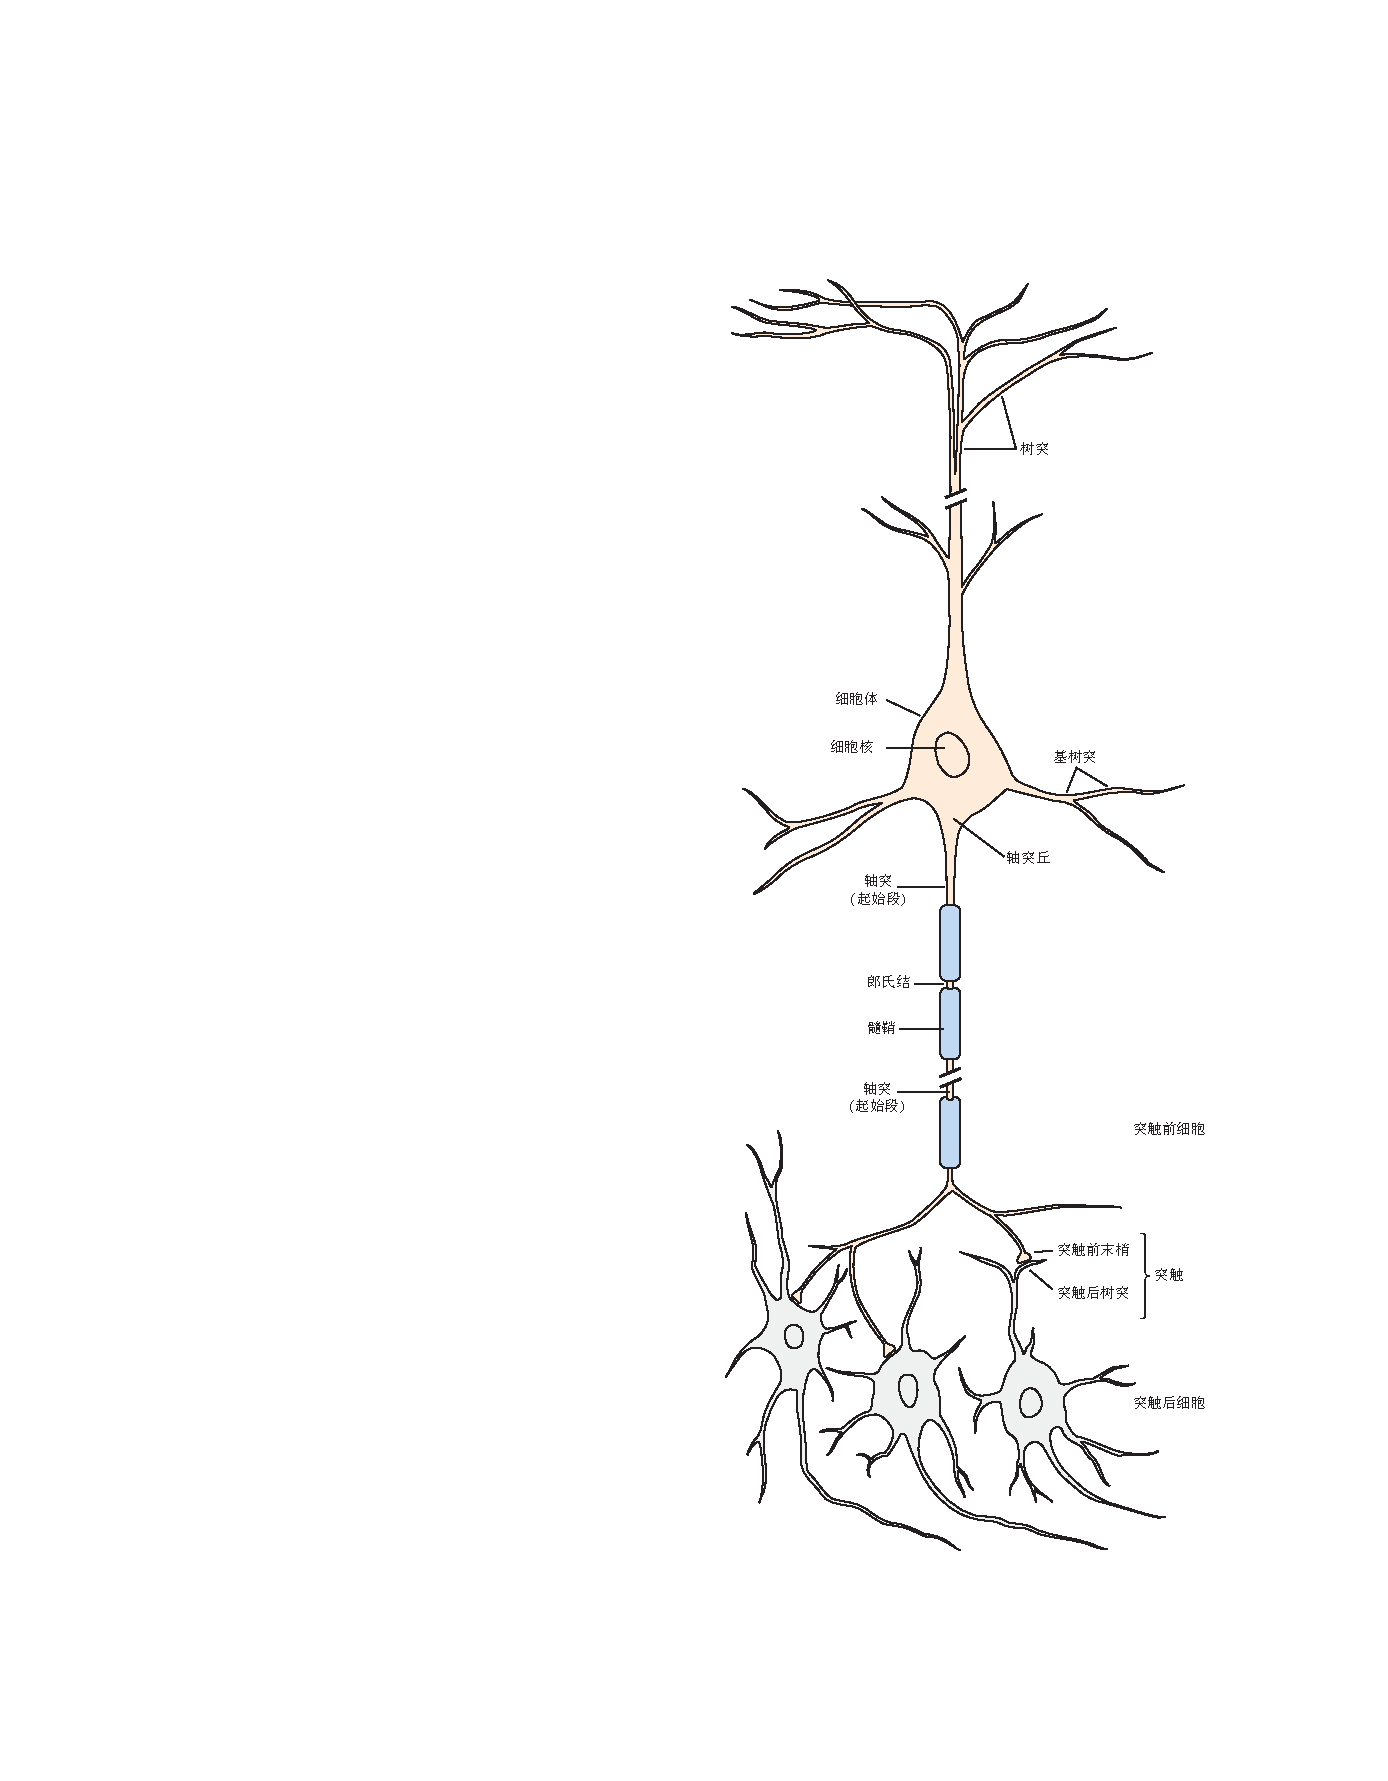
\includegraphics[width=0.5\linewidth]{chap03/fig_3_1}
	\caption{(右)神经元的结构。 
		脊椎动物神经系统中的大多数神经元有几个共同的主要特征。 
		细胞体包含细胞核,遗传信息的仓库,并产生两种类型的细胞过程:轴突和树突。 
		轴突是神经元的传递元件; 它们的长度差异很大,有些在体内延伸超过 1 米。 
		与细胞体的直径(50 μm 或更大)相比,中枢神经系统中的大多数轴突非常细(直径在 0.2 μm 和 20 μm 之间)。 
		许多轴突被一层脂肪髓鞘绝缘,该鞘在称为郎氏结的间隙处定期中断。 
		动作电位,即细胞的传导信号,在轴突的初始部分启动并传播到突触,突触是信号从一个神经元流向另一个神经元的部位。 
		突触前神经元的轴突分支将信号传递给突触后细胞。 
		单个轴突的分支可能与多达一千个突触后神经元形成突触。 
		顶端和基部树突与细胞体一起是神经元的输入元件,接收来自其他神经元的信号。}
	\label{fig:3_1}
\end{figure}


细胞体或胞体是细胞的代谢中心。 
它包括包含细胞基因的细胞核和内质网,内质网是合成细胞蛋白质的细胞核的延伸。 
细胞体通常产生两种过程:几个短的树突和一个长的管状轴突。 
树突以树状方式分支,是接收来自其他神经细胞的输入信号的主要装置。 
轴突通常在分支之前从细胞体延伸一定距离,使其能够将信号传递给许多目标神经元。
轴突可以在 0.1 毫米到 1 米的距离内传输电信号。 
这些电信号或动作电位在轴突起源附近的专门触发区域启动,称为初始段,动作电位从该区域以 1 至 100 m/s 的速度沿着轴突传播而不会失败或失真。 
沿轴突向下传播的动作电位的振幅保持恒定在 100 mV,因为动作电位是一种全有或全无的脉冲,它会沿着轴突定期再生(图 \ref{fig:3_2})。

\begin{figure}[htbp]
	\centering
	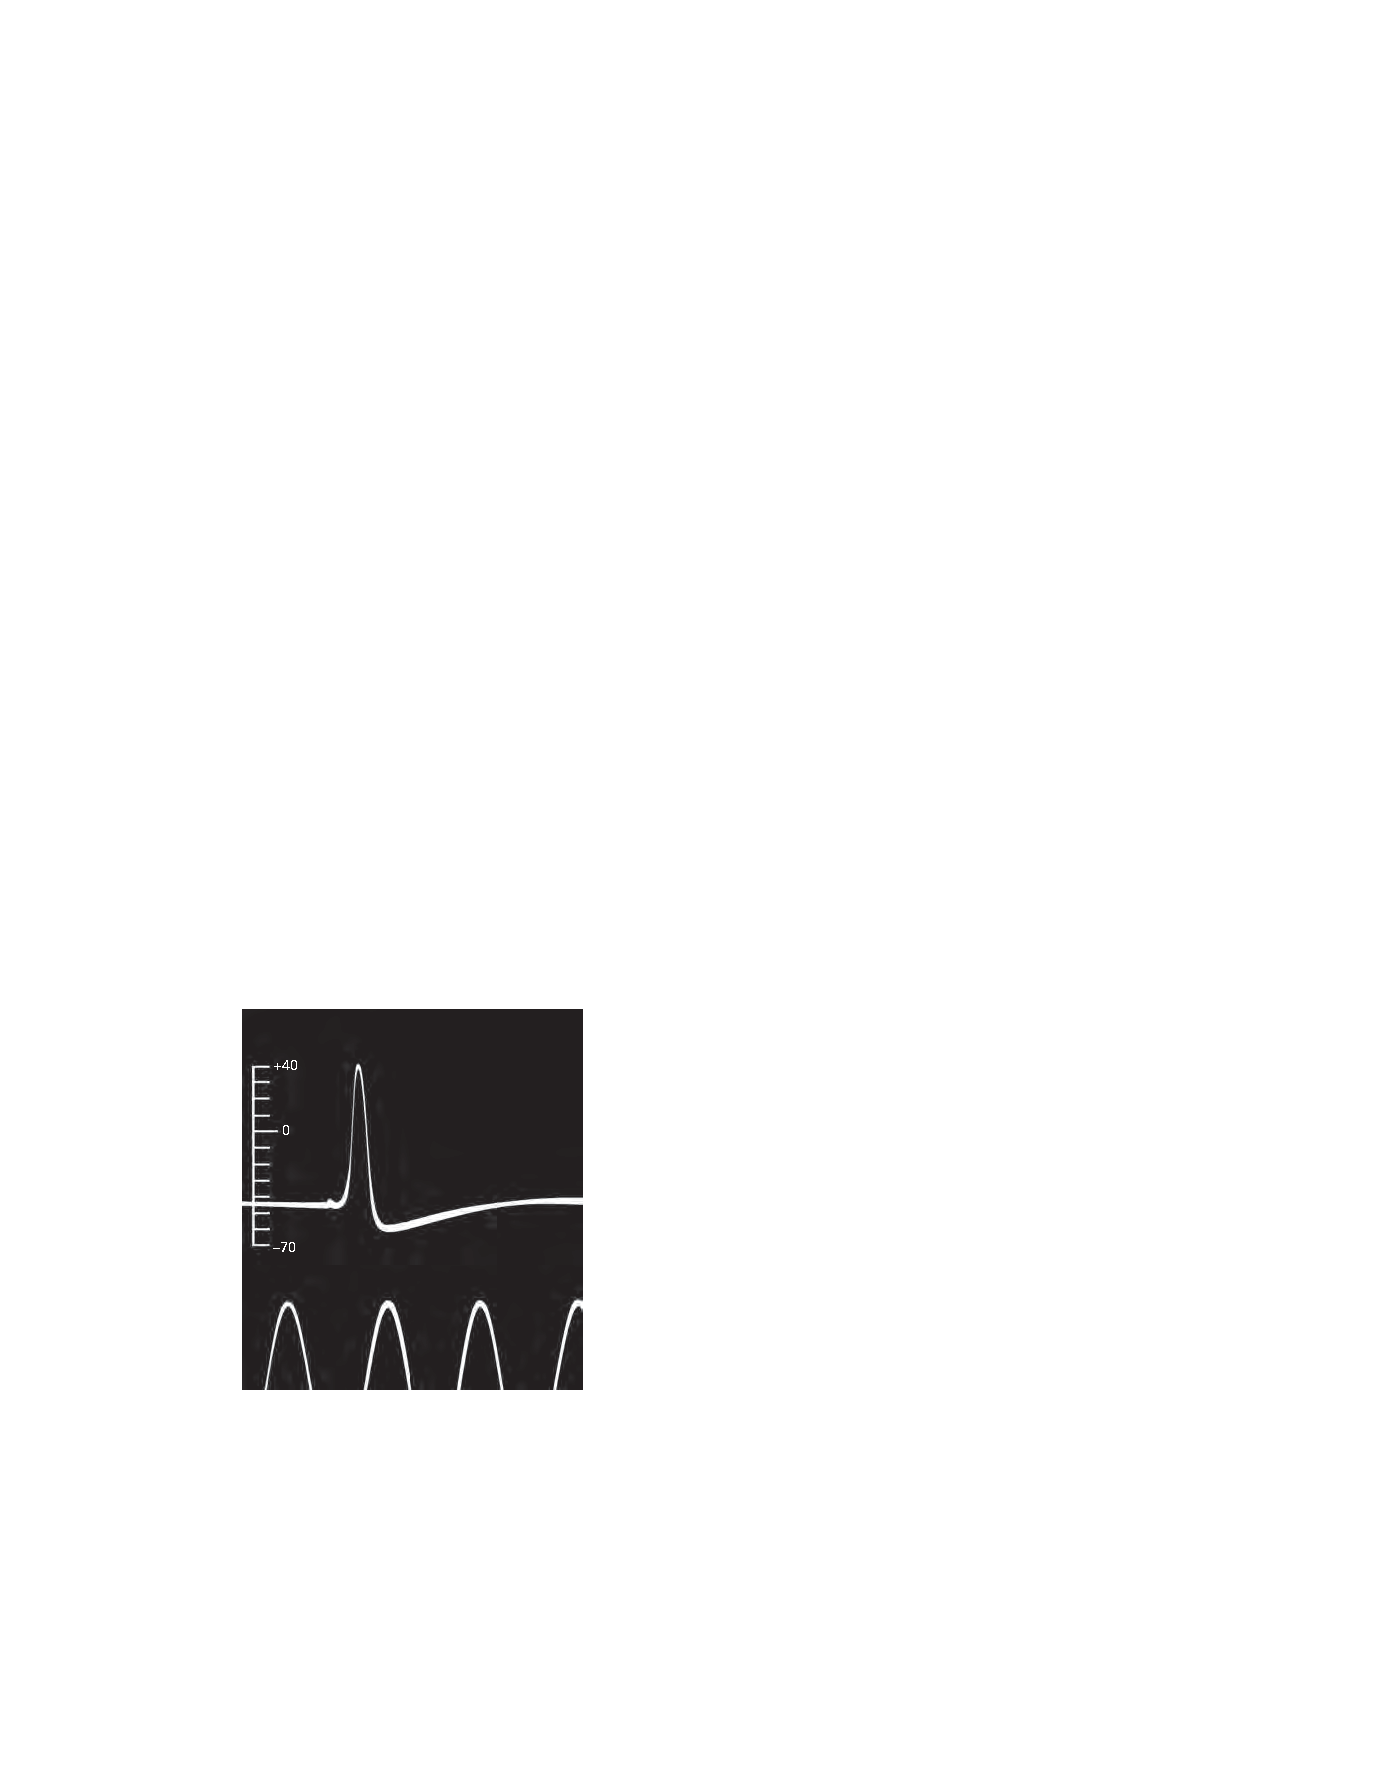
\includegraphics[width=0.5\linewidth]{chap03/fig_3_2}
	\caption{这一历史性追踪是首次公布的动作电位细胞内记录。 
		1939 年,艾伦·霍奇金 (Alan Hodgkin) 和安德鲁·赫胥黎 (Andrew Huxley) 使用充满海水的玻璃毛细管电极从乌贼巨型轴突上记录下来。 
		定时脉冲(底部)间隔 2 毫秒。 
		垂直刻度表示内部电极的电位,单位为毫伏,外面的海水被视为零电位。 
		(经许可转载自 Hodgkin 和 Huxley 1939。)}
	\label{fig:3_2}
\end{figure}


动作电位是大脑接收、分析和传递信息的信号。 
这些信号在整个神经系统中都是高度固定的,尽管它们是由环境中影响我们身体的各种事件引发的——从光到机械接触,从气味到压力波。 
传递视觉信息的生理信号与传递气味信息的生理信号相同。 
在这里,我们看到了大脑功能的一个关键原则:动作电位传递的信息类型不是由信号的形式决定的,而是由信号在大脑中传播的路径决定的。 
因此,大脑分析和解释通过特定路径传输的传入电信号的模式,进而创造我们的视觉、触觉、味觉、嗅觉和听觉感觉。


为了提高传导动作电位的速度,大轴突被包裹在脂质物质髓磷脂的绝缘鞘中。 
鞘被 Ranvier 节点定期中断,Ranvier 节点是轴突上再生动作电位的未绝缘点。 
(第 \ref{chap:chap7} 章和第 \ref{chap:chap8} 章详细讨论了髓鞘形成,第 \ref{chap:chap10} 章详细讨论了动作电位。)


在接近其末端时,轴突分成细枝,这些细枝在称为突触的特殊通讯区域与其他神经元联系。 
传递信号的神经细胞称为突触前细胞; 接收信号的细胞是突触后细胞。 
突触前细胞从其轴突分支的特殊扩大区域传输信号,称为突触前末梢或神经末梢。 
突触前和突触后细胞被一个非常狭窄的空间隔开,即突触间隙。 
大多数突触前终端终止于突触后神经元的树突,但有些也终止于细胞体,或者较少见的是终止于突触后细胞轴突的起点或末端(见图 \ref{fig:3_1})。 
一些突触前神经元会激发它们的突触后靶细胞; 其他突触前神经元抑制它们的靶细胞。


神经元学说(第 \ref{chap:chap1} 章)认为每个神经元都是一个离散的细胞,其细胞体具有独特的过程,并且神经元是神经系统的信号单元。 
回想起来,很难体会到科学家最初提出这个基本想法时有多难接受。 
与其他组织的细胞具有简单的形状并适合光学显微镜的单个视野不同,神经细胞具有复杂的形状。 
树突的复杂模式和一些轴突看似无穷无尽的过程使得在这些元素之间建立关系变得极其困难。 
即使在解剖学家 Jacob Schleiden 和 Theodor Schwann 于 1830 年代初期提出细胞理论之后——细胞是所有生命物质的结构单元的观点成为生物学的中心教条——大多数解剖学家也不接受细胞理论应用于 大脑,他们认为大脑是一个连续的、网状的网状结构,由非常薄的过程组成。


神经元的连贯结构直到 19 世纪后期才变得清晰,当时 Ramón y Cajal 开始使用高尔基体引入的银染法。 
这种方法至今仍在使用,它有两个优点。 
首先,以一种不为人知的随机方式,银溶液仅染色任何特定大脑区域中约 1\% 的细胞,这使得独立于其相邻神经元检查单个神经元成为可能。 
其次,确实吸收了染色剂的神经元被完整地描绘出来,包括细胞体、轴突和完整的树突树。 
染色表明神经元之间没有细胞质连续性,卡哈尔预言性地正确地得出结论,即使在两个细胞之间的突触处也没有连续性。


Ramón y Cajal 将高尔基的方法应用于许多动物和人类的胚胎神经系统。 
通过检查神经系统几乎每个区域的神经元结构,他可以描述神经细胞的类别并绘制出许多神经细胞之间的精确联系。 
通过这种方式,除了神经元学说之外,Ramón y Cajal 还推导出了另外两个神经组织原理,这两个原理在研究神经系统的交流方面特别有价值。


其中第一个是动态极化原理,它指出神经细胞内的电信号仅沿一个方向流动:
从神经元的突触后部位(通常是树突和细胞体)到轴突的触发区域。 
从那里,动作电位沿着轴突的整个长度传播到其末端。 
在迄今为止研究的大多数神经元中,电信号实际上沿着轴突沿一个方向传播。


Ramón y Cajal 提出的第二个原则,即连接特异性,指出神经细胞在网络形成过程中不会随机相互连接,而是在特定接触点与某些突触后靶细胞而非其他突触后靶细胞建立特定连接。 
动态极化和连接特异性的原理是现代细胞连接主义研究大脑方法的基础。


Ramón y Cajal 也是最先认识到一种神经元与另一种神经元最大区别的特征是形式,特别是细胞体产生的过程的数量。 
因此,神经元分为三大类:单极、双极和多极。


单极神经元是最简单的,因为它们只有一个初级过程,通常会产生许多分支。 
一个分支作为轴突; 其他分支充当接收结构(图 \ref{fig:3_3}A)。 
这些细胞在无脊椎动物的神经系统中占主导地位; 
在脊椎动物中,它们发生在自主神经系统中。

\begin{figure}[htbp]
	\centering
	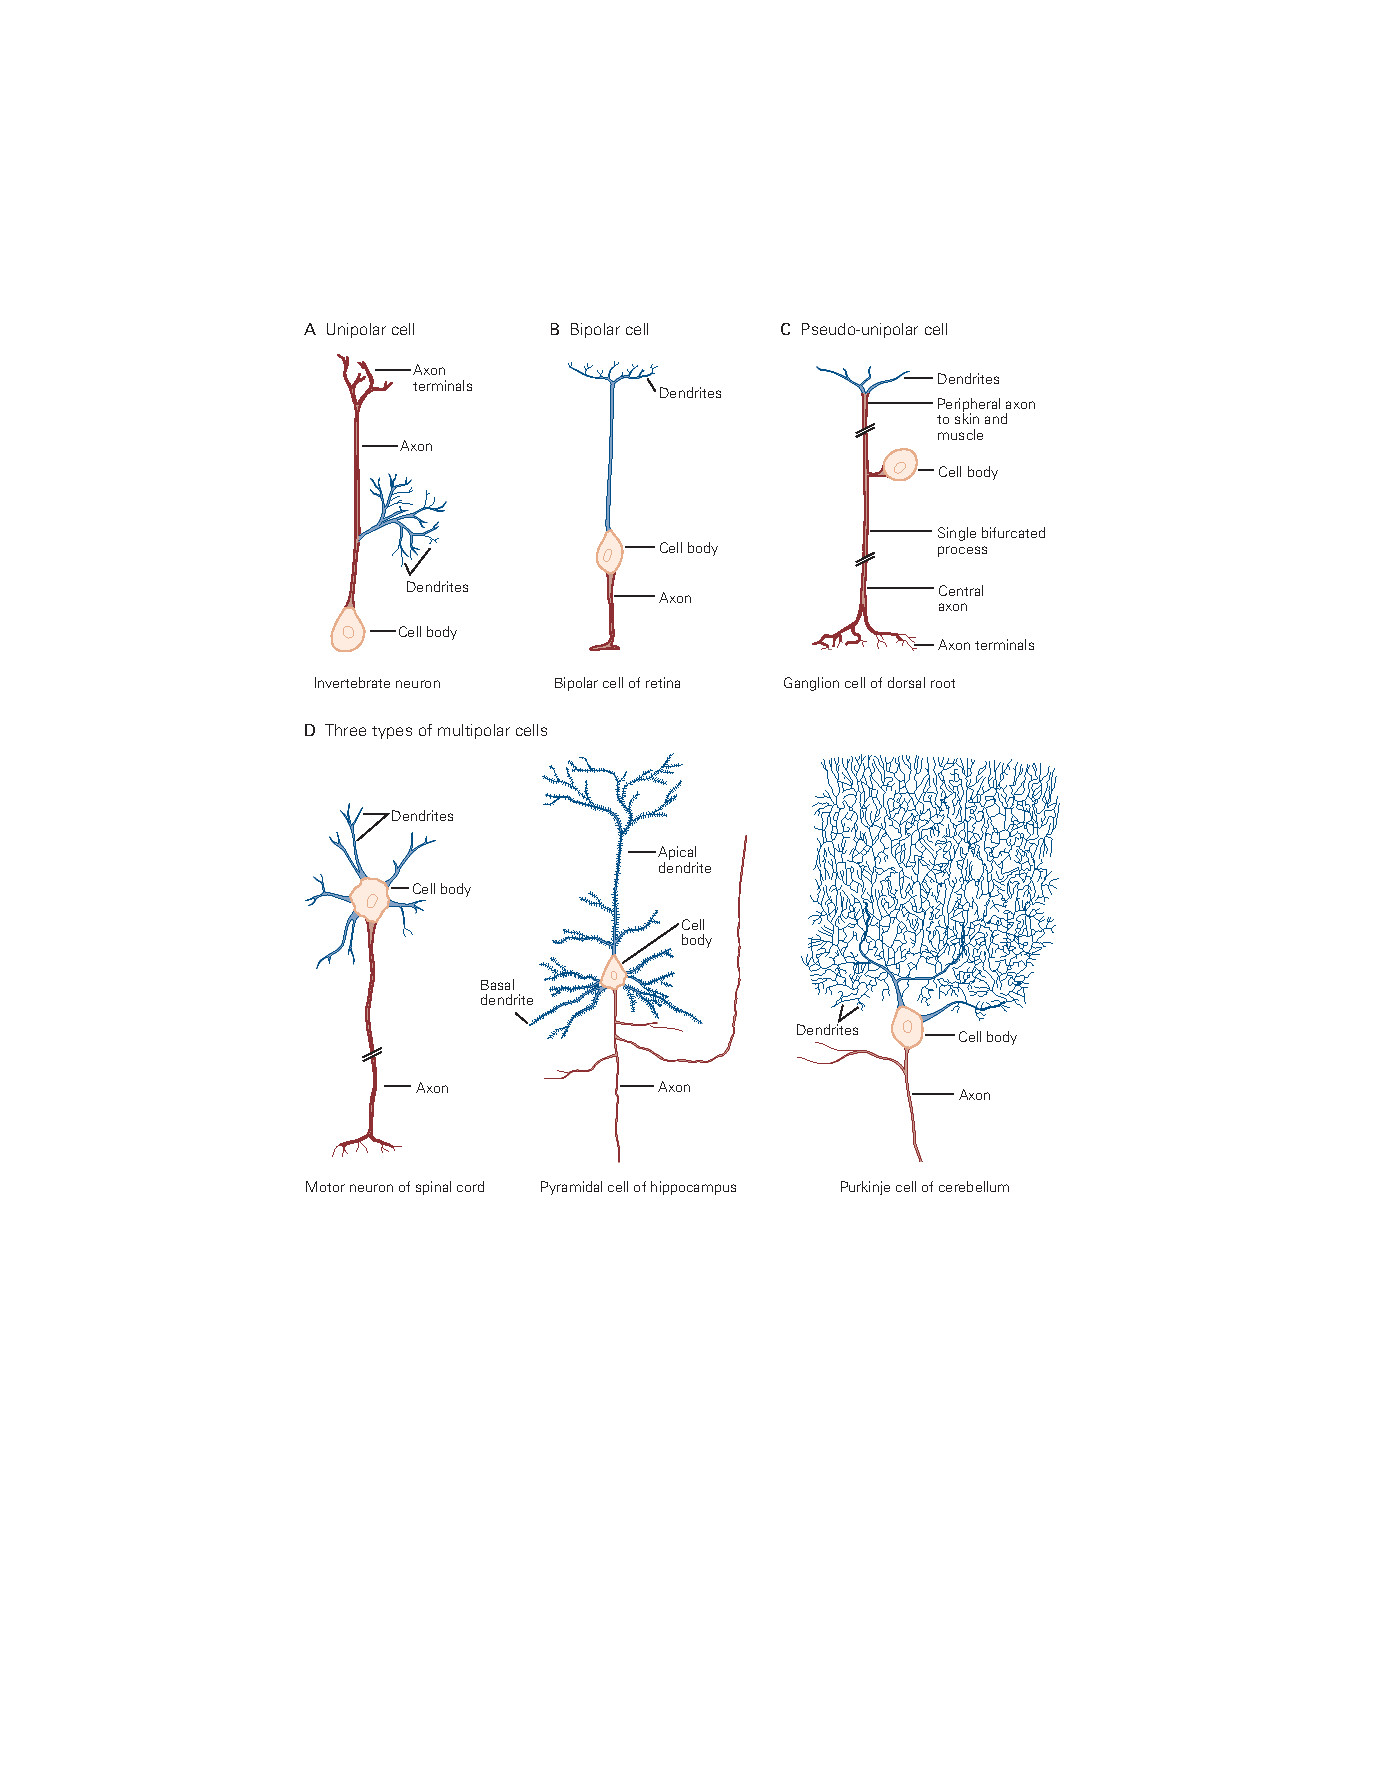
\includegraphics[width=0.9\linewidth]{chap03/fig_3_3}
	\caption{根据源自细胞体的过程的数量,神经元分为单极、双极或多极。 
		\textbf{A.} 单极电池有一个从电池发出的过程。 
		不同的部分作为接受表面或释放终端。 
		单极细胞是无脊椎动物神经系统的特征。 
		\textbf{B.} 双极细胞有两种功能专门化的过程。 
		树突接收电信号,轴突将信号传递给其他细胞。 
		\textbf{C.} 伪单极细胞是双极细胞的变体,将体感信息传递到脊髓。 
		在发育过程中,胚胎双极细胞的两个过程融合并作为一个过程从细胞体中出现,该过程具有两个功能不同的部分。 
		两个部分都起轴突的作用; 一个延伸到外周皮肤或肌肉,另一个延伸到中央脊髓\cite{ross2006histology}。
		\textbf{D.} 多极细胞具有单个轴突和许多树突。 
		它们是哺乳动物神经系统中最常见的神经元类型。 
		三个例子说明了这些细胞的巨大多样性。 
		脊髓运动神经元支配骨骼肌纤维。
		锥体细胞具有大致三角形的细胞体;
		树突从顶点(顶端树突)和基部(基底树突)出现。 
		锥体细胞存在于海马体和整个大脑皮层中。 
		小脑的浦肯野细胞的特征是丰富而广泛的树突状树,可容纳大量突触输入\cite{ross2006histology}。}
	\label{fig:3_3}
\end{figure}


双极神经元有一个椭圆形的体细胞,它产生两个不同的过程:
一个树突结构接收来自其他神经元的信号,一个轴突将信息传递给中枢神经系统(图 \ref{fig:3_3}B)。 
许多感觉细胞是双极的,包括视网膜和鼻子的嗅觉上皮细胞。 
向脊髓传递触觉、压力和疼痛信号的受体神经元最初发育为双极细胞,但两个细胞过程融合成一个单一的连续结构,从细胞体的一个点出现,树突被赋予了 使它成为轴突的特化。 
在这些所谓的伪单极细胞中,一个轴突将信息从皮肤、关节和肌肉中的感觉受体传递到细胞体,而另一个轴突将此感觉信息传递到脊髓(图 \ref{fig:3_3}C)。


多极神经元在脊椎动物的神经系统中占主导地位。 
它们通常有一个轴突和许多从细胞体周围不同点出现的树突结构(图 \ref{fig:3_3}D)。 
多极细胞的形状差异很大,尤其是轴突的长度以及树突分支的范围、尺寸和复杂性。 
通常,分支的程度与其他神经元与其进行的突触接触的数量相关。 
一个树突数量相对较少的脊髓运动神经元接受大约 10,000 个接触——1,000 个在细胞体上,9,000 个在树突上。 
在小脑的浦肯野细胞中,树突树更大更茂密,接受多达一百万次接触!


神经细胞也分为三个主要功能类别:感觉神经元、运动神经元和中间神经元。 
感觉神经元将信息从身体的外围传感器传送到神经系统,以达到感知和运动协调的目的。 
一些初级感觉神经元称为传入神经元,这两个术语可以互换使用。 
术语传入(传向中枢神经系统)适用于从外围到达中枢神经系统的所有信息,无论该信息是否导致感觉。 
术语“感觉”是指那些将信息从感觉上皮细胞、关节感觉受体或肌肉传递到中枢神经系统的传入神经元,但该概念已扩展到包括初级和次级皮层区域中的神经元,这些神经元对变化做出反应 感觉特征,例如物体在空间中的位移、声音频率的变化或头部的角旋转(通过耳朵中的前庭器官),甚至像面部这样复杂的东西。


传出一词适用于从中枢神经系统向运动器官传递的所有信息,无论这些信息是否导致行动。 
运动神经元将命令从大脑或脊髓传递到肌肉和腺体(传出信息)。 
运动神经元(或运动神经元)的传统定义是激发肌肉的神经元,但运动神经元的名称现在包括不直接支配肌肉但间接命令动作的其他神经元。 
运动神经元和感觉神经元的一个有用特征是它们对神经系统外事物的时间保真度。 
它们的活动跟上外部刺激和身体肌肉组织施加的动力的变化。 
感觉神经元为大脑提供数据,而运动神经元将观念转化为实践。 
它们共同构成了我们与世界的界面。


中间神经元包含最多的功能类别,并细分为两类:中继和本地。 
中继或投射中间神经元具有长轴突,可在相当长的距离内将信号从一个大脑区域传送到另一个大脑区域。 
局部中间神经元的轴突较短,因为它们与局部回路中附近的神经元形成连接。 
由于几乎每个神经元都可以被视为中间神经元,因此该术语通常用于区分投射到局部回路中另一个神经元的神经元和投射到单独神经结构的神经元。 
该术语有时也用作抑制性神经元的简写,特别是在皮层回路的研究中,但为了清楚起见,应在适当的时候使用术语抑制性中间神经元。


每个功能分类可以进一步细分。 
感觉系统中间神经元可以根据它们响应的感觉刺激的类型进行分类; 
这些最初的分类可以根据位置、密度、大小以及基因表达模式进一步细分。 
事实上,由于\textit{信使核糖核酸}序列分析的进步使单个神经元的分子谱分析成为可能,我们对神经元复杂性的看法正在迅速发展。 
此类分析最近揭示了神经元类型的异质性比以前认为的要大得多(图 \ref{fig:3_4})。

\begin{figure}[htbp]
	\centering
	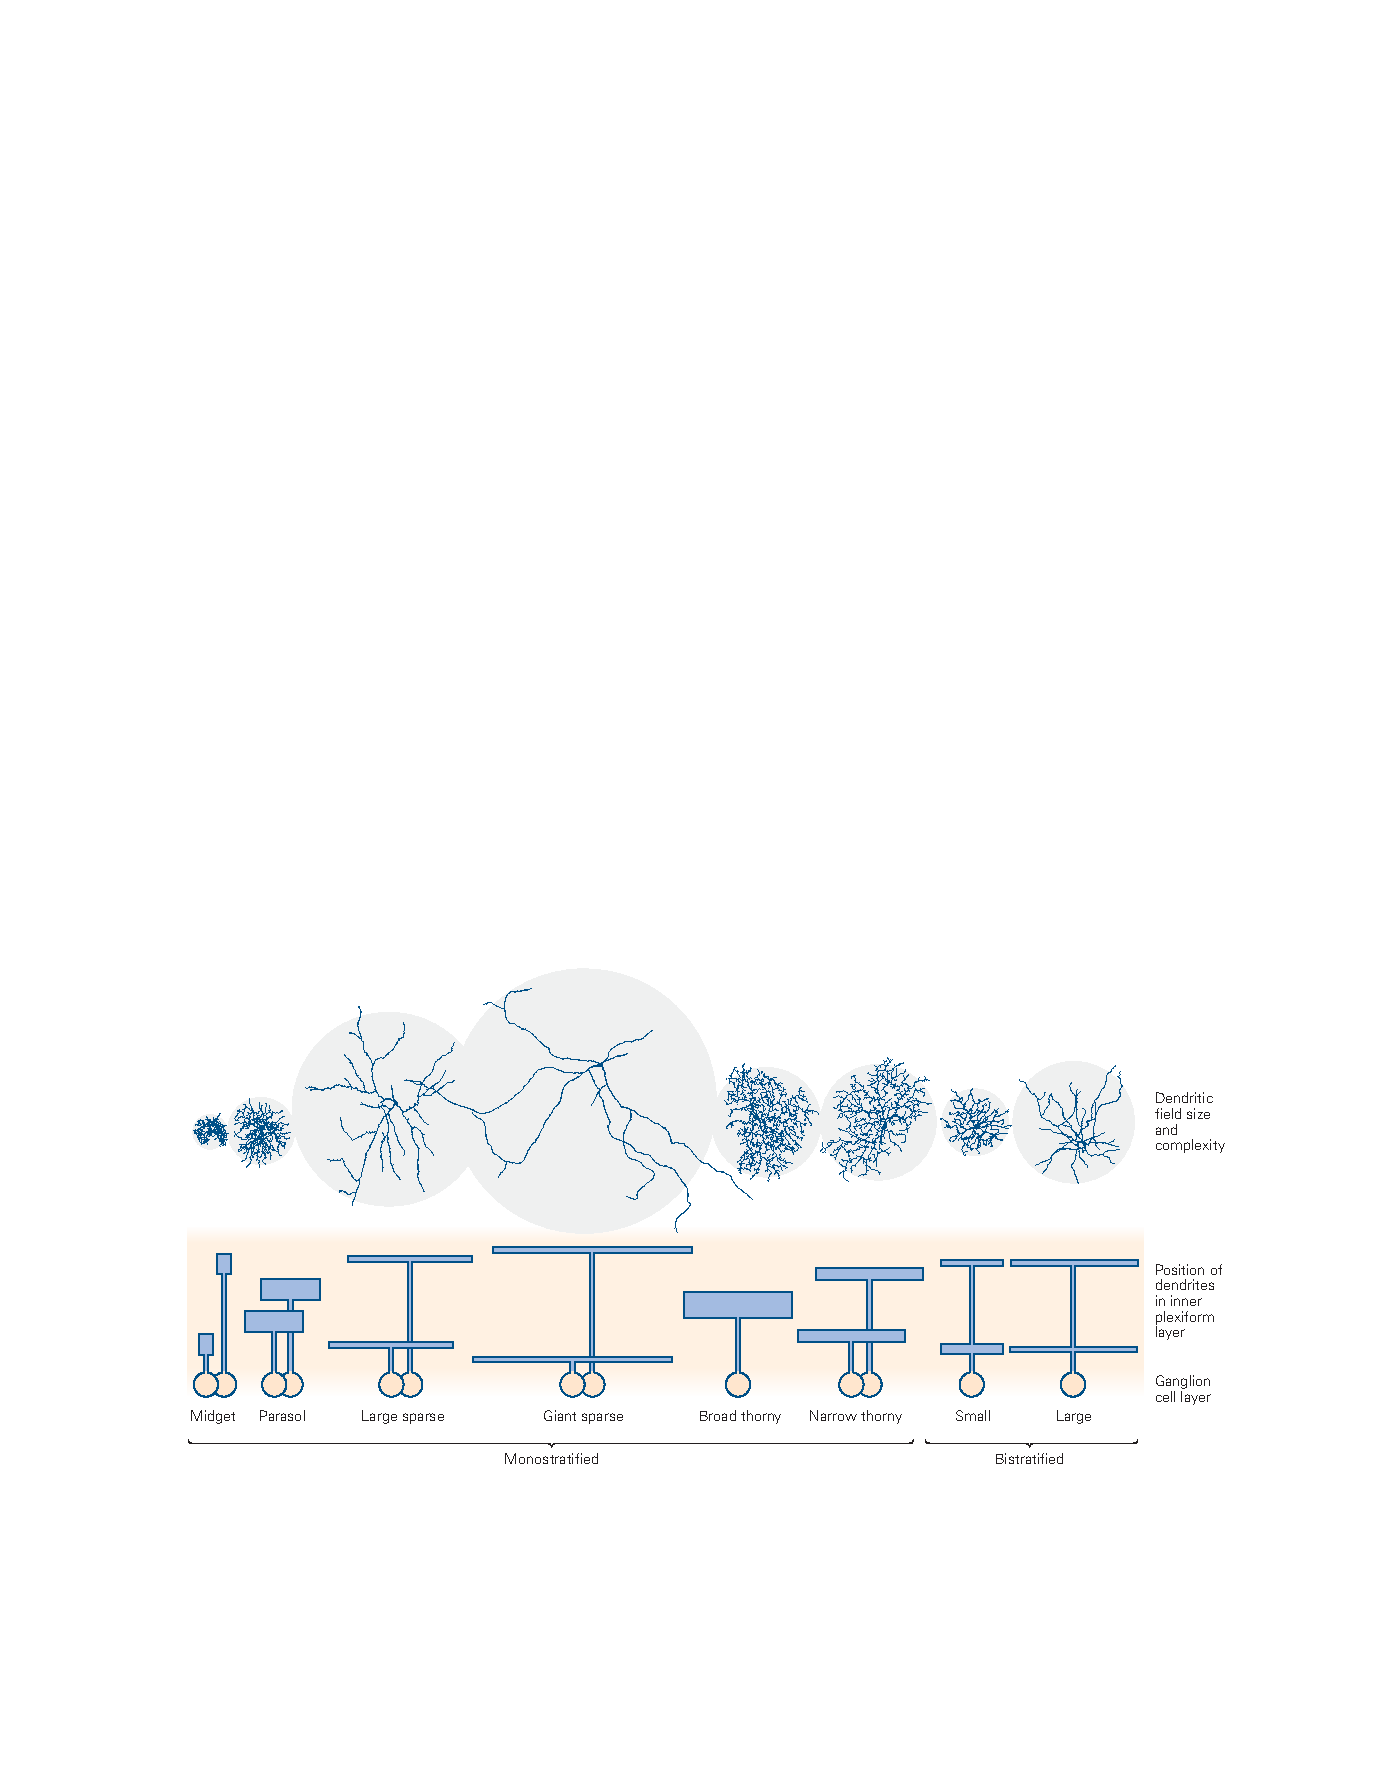
\includegraphics[width=1.0\linewidth]{chap03/fig_3_4}
	\caption{感觉神经元可以细分为功能不同的组。 
		例如,至少有 13 种类型的视网膜神经节细胞是根据它们的树突的大小和形状以及它们接收输入信号的视网膜深度来区分的。 
		内丛状层包含视网膜中间神经元(双极和无长突细胞)和神经节细胞之间的连接。 
		(经许可转载自 Dacey 等人,2003 年。版权所有 © 2003 Elsevier。)}
	\label{fig:3_4}
\end{figure}


\subsection{神经胶质细胞支持神经细胞}
神经胶质细胞的数量远远超过神经元——在脊椎动物中枢神经系统中,神经胶质细胞的数量是神经元的 2 到 10 倍。 
尽管这些细胞的名称源自希腊语中的胶水,但胶质细胞通常不会将神经细胞聚集在一起。 
相反,它们围绕着神经元的细胞体、轴突和树突。 
胶质细胞在形态上不同于神经元; 它们不形成树突和轴突。


胶质细胞在功能上也有所不同。 
尽管它们来自相同的胚胎前体细胞,但它们不具有与神经元相同的膜特性,因此不能被电激发。 
因此,它们不直接参与电信号传递,这是神经细胞的功能。 
然而,它们在允许电信号沿着神经元的轴突快速移动方面发挥了作用,而且它们似乎在引导早期发育过程中的连接以及稳定通过学习发生的神经元之间新的或改变的连接方面发挥了重要作用。 
在过去的十年中,人们对胶质细胞的多种功能的兴趣有所增加,它们的特征已经从支持细胞转变为神经元的功能伙伴(第 \ref{chap:chap7} 章)。


\section{每个神经细胞都是调节特定行为的回路的一部分}
每一种行为都由一组特定的相互连接的神经元介导,而每
一个神经元的行为功能都取决于它与其他神经元的联系。 一个简单的行为,膝跳反射,将说明这一点。 
当身体的短暂不平衡拉伸腿部股四头肌伸肌时,反射开始。 
这种拉伸会产生传送给运动神经元的感觉信息,而运动神经元又会向伸肌发出收缩命令,从而恢复平衡。


这种反射在临床上用于测试神经的完整性以及反射幅度(或增益)的脑脊髓控制。 
潜在的机制很重要,因为它可以维持股四头肌的正常张力,并防止我们的膝盖在站立或行走时屈曲。 
股四头肌的肌腱,一种移动小腿的伸肌,通过髌骨(膝盖骨)的肌腱附着在胫骨上。 
轻敲髌骨正下方的肌腱可以拉伸股四头肌。 
这种拉伸启动股四头肌的反射性收缩,产生熟悉的膝跳。 
通过增加选定肌肉群的张力,牵张反射改变腿的位置,突然向外伸展(图 \ref{fig:3_5})。

\begin{figure}[htbp]
	\centering
	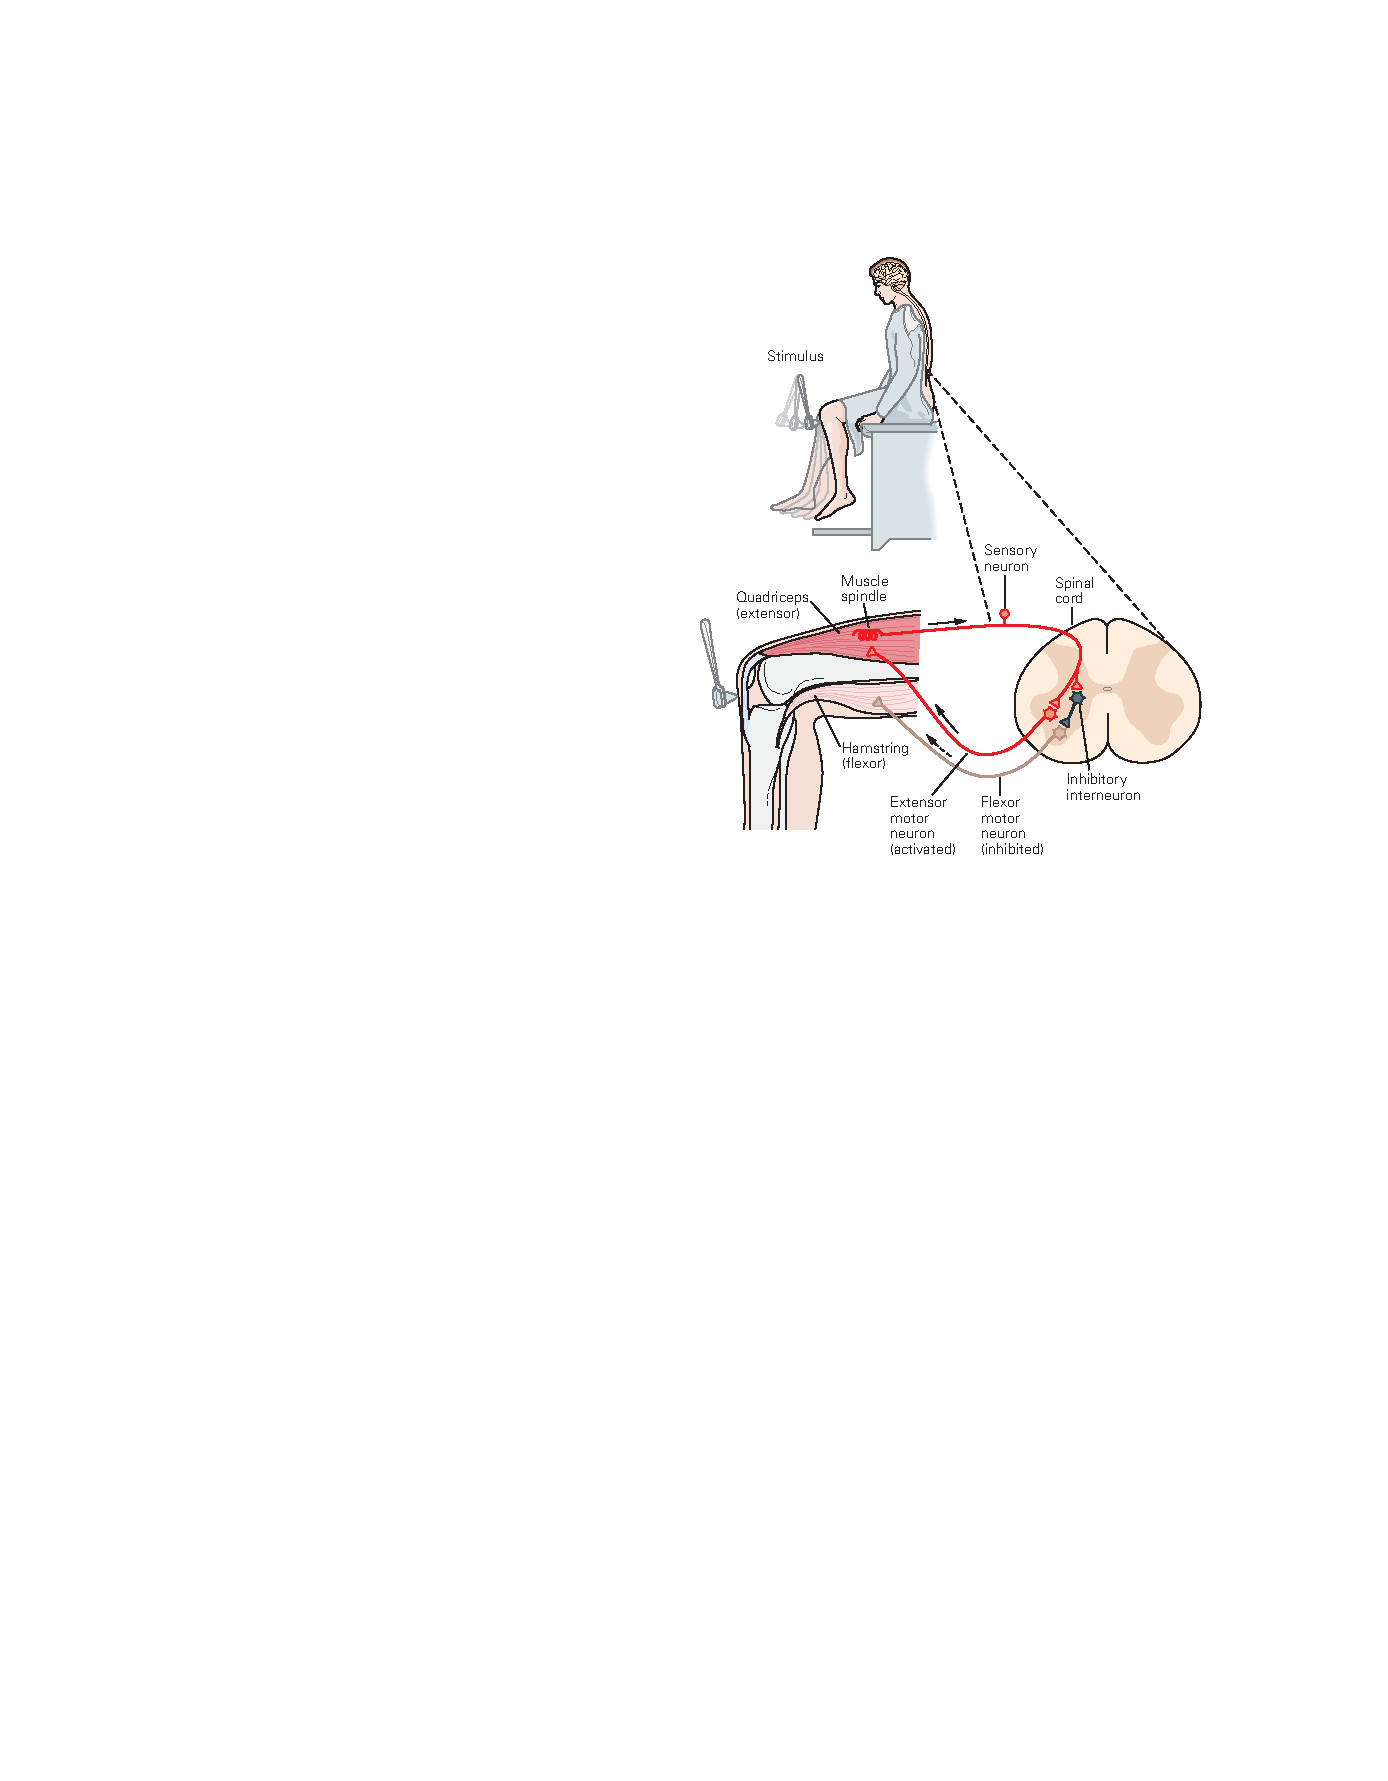
\includegraphics[width=0.5\linewidth]{chap03/fig_3_5}
	\caption{膝跳反射由感觉和运动神经元组成的简单回路控制。 
		用反射锤轻敲膝盖骨,拉动股四头肌的肌腱,股四头肌是延伸小腿的肌肉。
		当肌肉因肌腱的牵拉而伸展时,有关肌肉变化的信息会通过感觉神经元传送到中枢神经系统。 
		在脊髓中,感觉神经元与收缩股四头肌(被拉伸的肌肉)的伸肌运动神经元形成兴奋性突触。 
		感觉神经元通过中间神经元间接作用,抑制屈肌运动神经元,否则这些神经元会收缩相对的腿筋肌肉。 
		这些动作结合起来产生反射行为。 
		在图中,每个伸肌和屈肌运动神经元代表许多细胞群。}
	\label{fig:3_5}
\end{figure}


参与膝跳反射的感觉神经元的细胞体聚集在背根神经节的脊髓附近。 
它们是伪单极细胞; 每个细胞轴突的一个分支延伸到周围的股四头肌,而另一个延伸到脊髓的中央。 
支配股四头肌的分支与拉伸敏感受体(肌梭)接触,并在肌肉拉伸时兴奋。 
到达脊髓的分支与支配股四头肌并控制其收缩的运动神经元形成兴奋性连接。 
该分支还联系抑制控制相对屈肌的运动神经元的局部中间神经元(图 \ref{fig:3_5})。 
尽管这些局部中间神经元本身不参与牵张反射的产生,但它们通过协调相反肌肉群的动作来增加反射的稳定性。 
因此,产生牵张反射的电信号携带四种信息:

1. 感觉信息从肌肉传递到中枢神经系统(脊髓)。

2. 来自中枢神经系统的运动命令被发送到进行膝跳的肌肉。

3. 向支配相反肌肉的运动神经元发出抑制性命令。

4. 与膝跳有关的局部神经元活动的信息被发送到中枢神经系统的更高中枢,允许大脑同时或依次协调不同的行为。

此外,大脑断言对反射的上下文相关控制以调整其增益。 
例如,当我们跑步时,腿筋肌肉会弯曲膝盖,从而拉伸股四头肌。 
大脑和脊髓抑制牵张反射,使股四头肌放松。 
当这些下行路径被破坏时,就像在某些划水动作中一样,反射被放大并且关节变得僵硬。


仅仅拉伸一块肌肉,股四头肌,就会激活数百个感觉神经元,每个神经元与 45 到 50 个运动神经元直接接触。 
这种连接模式,其中一个神经元激活许多目标细胞,称为发散(图 \ref{fig:3_6}A)。 
它在神经系统的输入阶段尤为常见; 通过将其信号分配给许多靶细胞,单个神经元可以发挥广泛而多样的影响。 
相反,膝跳回路中的单个运动细胞从大约 130 个感觉细胞接收 200 到 450 个输入触点。 
这种连接模式称为收敛(图 \ref{fig:3_6}B)。 
它在神经系统的输出阶段很常见; 从许多感觉神经元接收信息的目标运动细胞能够整合来自许多来源的信息。 
每个感觉神经元输入产生相对较弱的兴奋,因此收敛也确保只有当足够数量的感觉神经元一起被激活时,运动神经元才会被激活。


\begin{figure}[htbp]
	\centering
	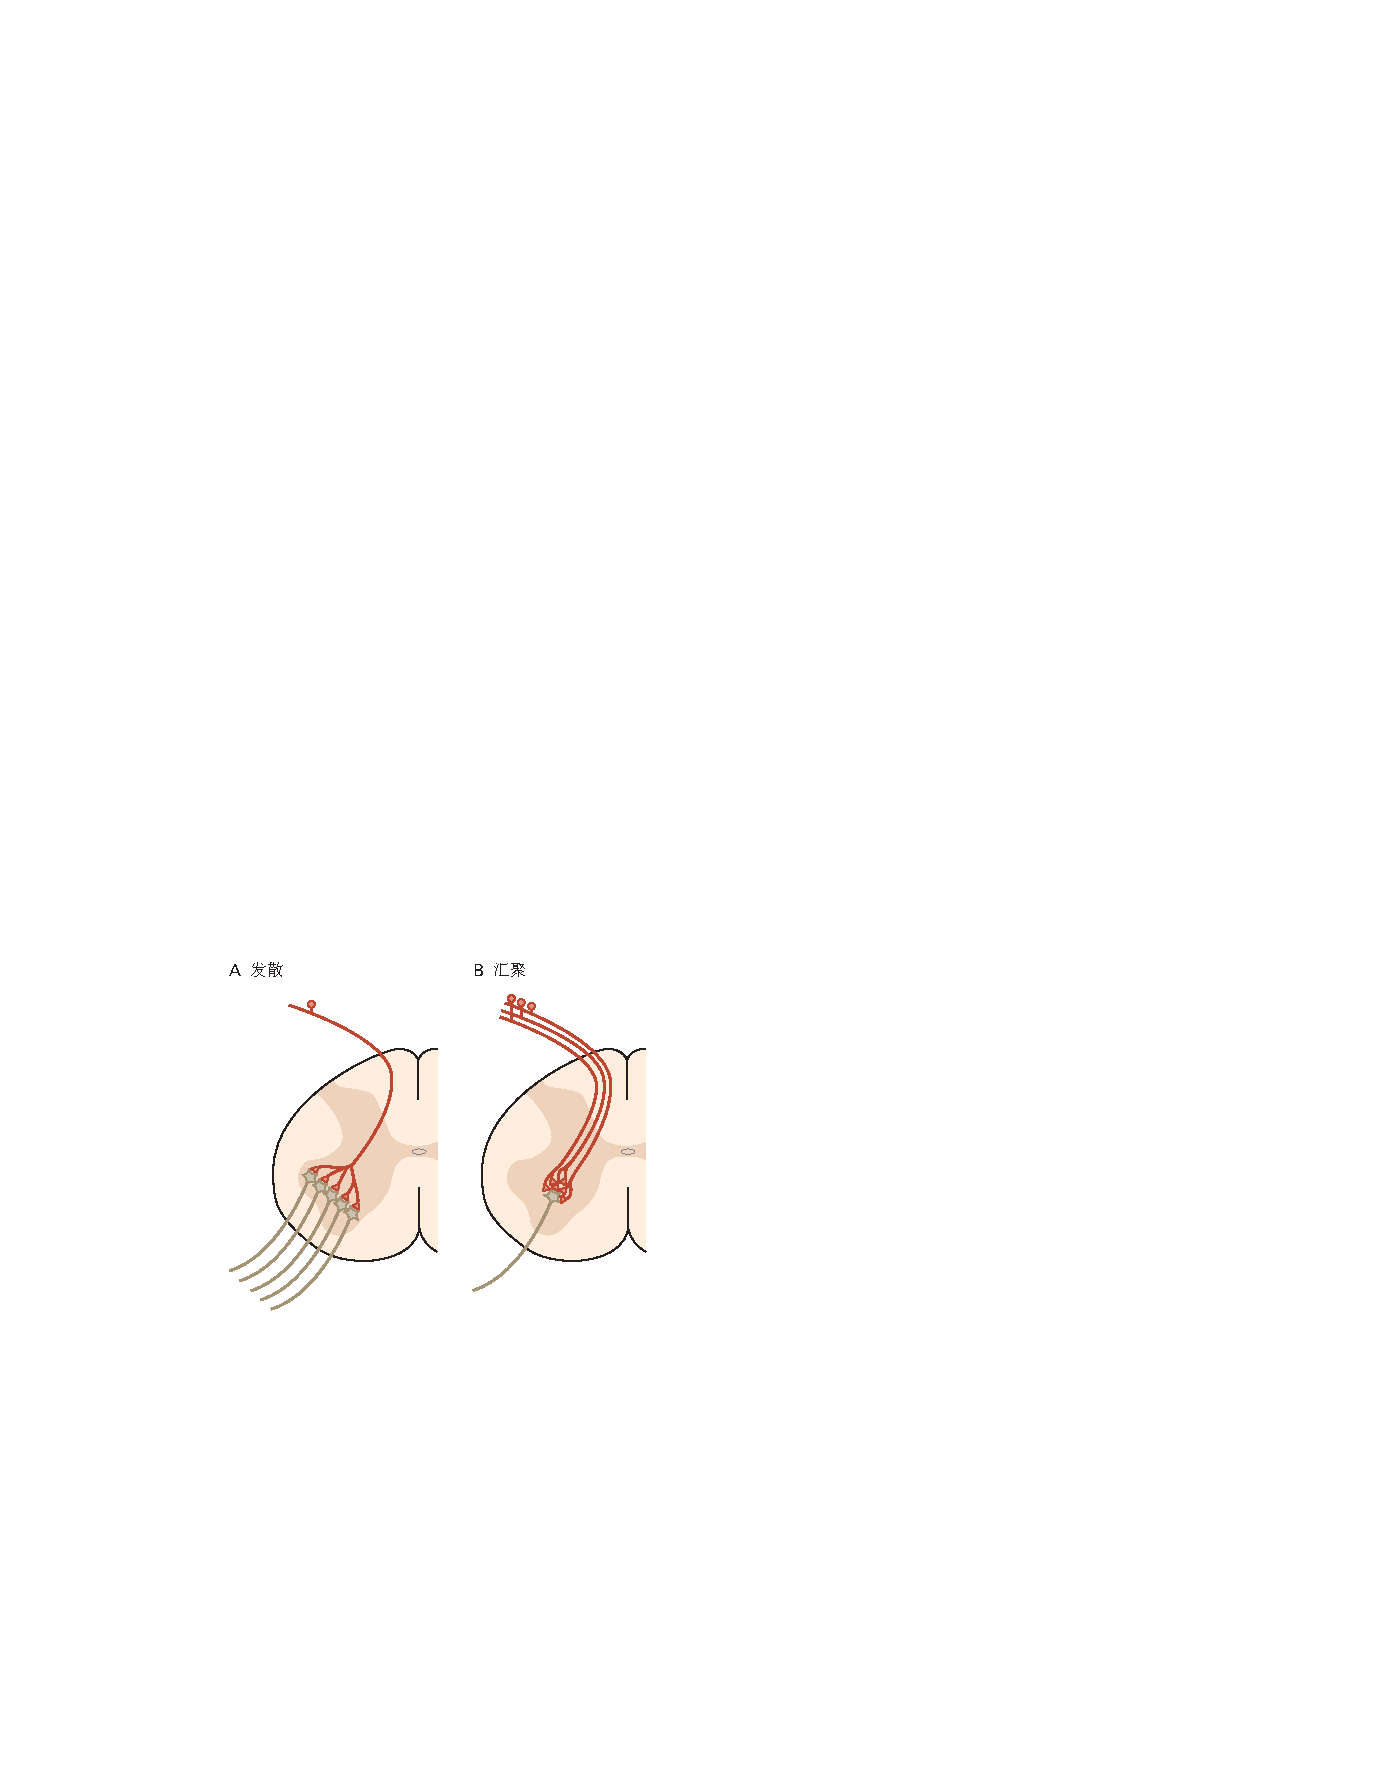
\includegraphics[width=0.5\linewidth]{chap03/fig_3_6}
	\caption{发散和会聚的神经元连接是大脑的一个关键组织特征。 
		A. 在感觉系统中,每个受体神经元通常与代表第二阶段处理的几个神经元联系。 
		在随后的处理阶段,传入的连接更加分散。 
		这使得来自单个站点的感觉信息可以更广泛地分布在脊髓和大脑中。 
		B. 相比之下,运动神经元是逐渐融合连接的目标。 
		通过这种安排,需要来自许多突触前细胞的输入来激活运动神经元。}
	\label{fig:3_6}
\end{figure}


诸如膝跳反射之类的牵张反射是由在兴奋性突触处连接的两类神经元产生的一种简单行为。 
但并非大脑中的所有重要信号都是兴奋性的。 
许多神经元会产生抑制信号,从而降低放电的可能性。 
即使在简单的膝跳反射中,感觉神经元也会产生兴奋性和抑制性连接。 
腿部伸肌中的兴奋性连接会导致这些肌肉收缩,而与抑制性中间神经元的连接会阻止拮抗性屈肌收缩。 
回路的这个特性是前馈抑制的一个例子(图~\ref{fig:3_7}A)。 
在膝跳反射中,前馈抑制是相互的,确保屈肌和伸肌通路始终相互抑制,以便只招募适合运动的肌肉,而不是那些反对运动的肌肉。

\begin{figure}[htbp]
	\centering
	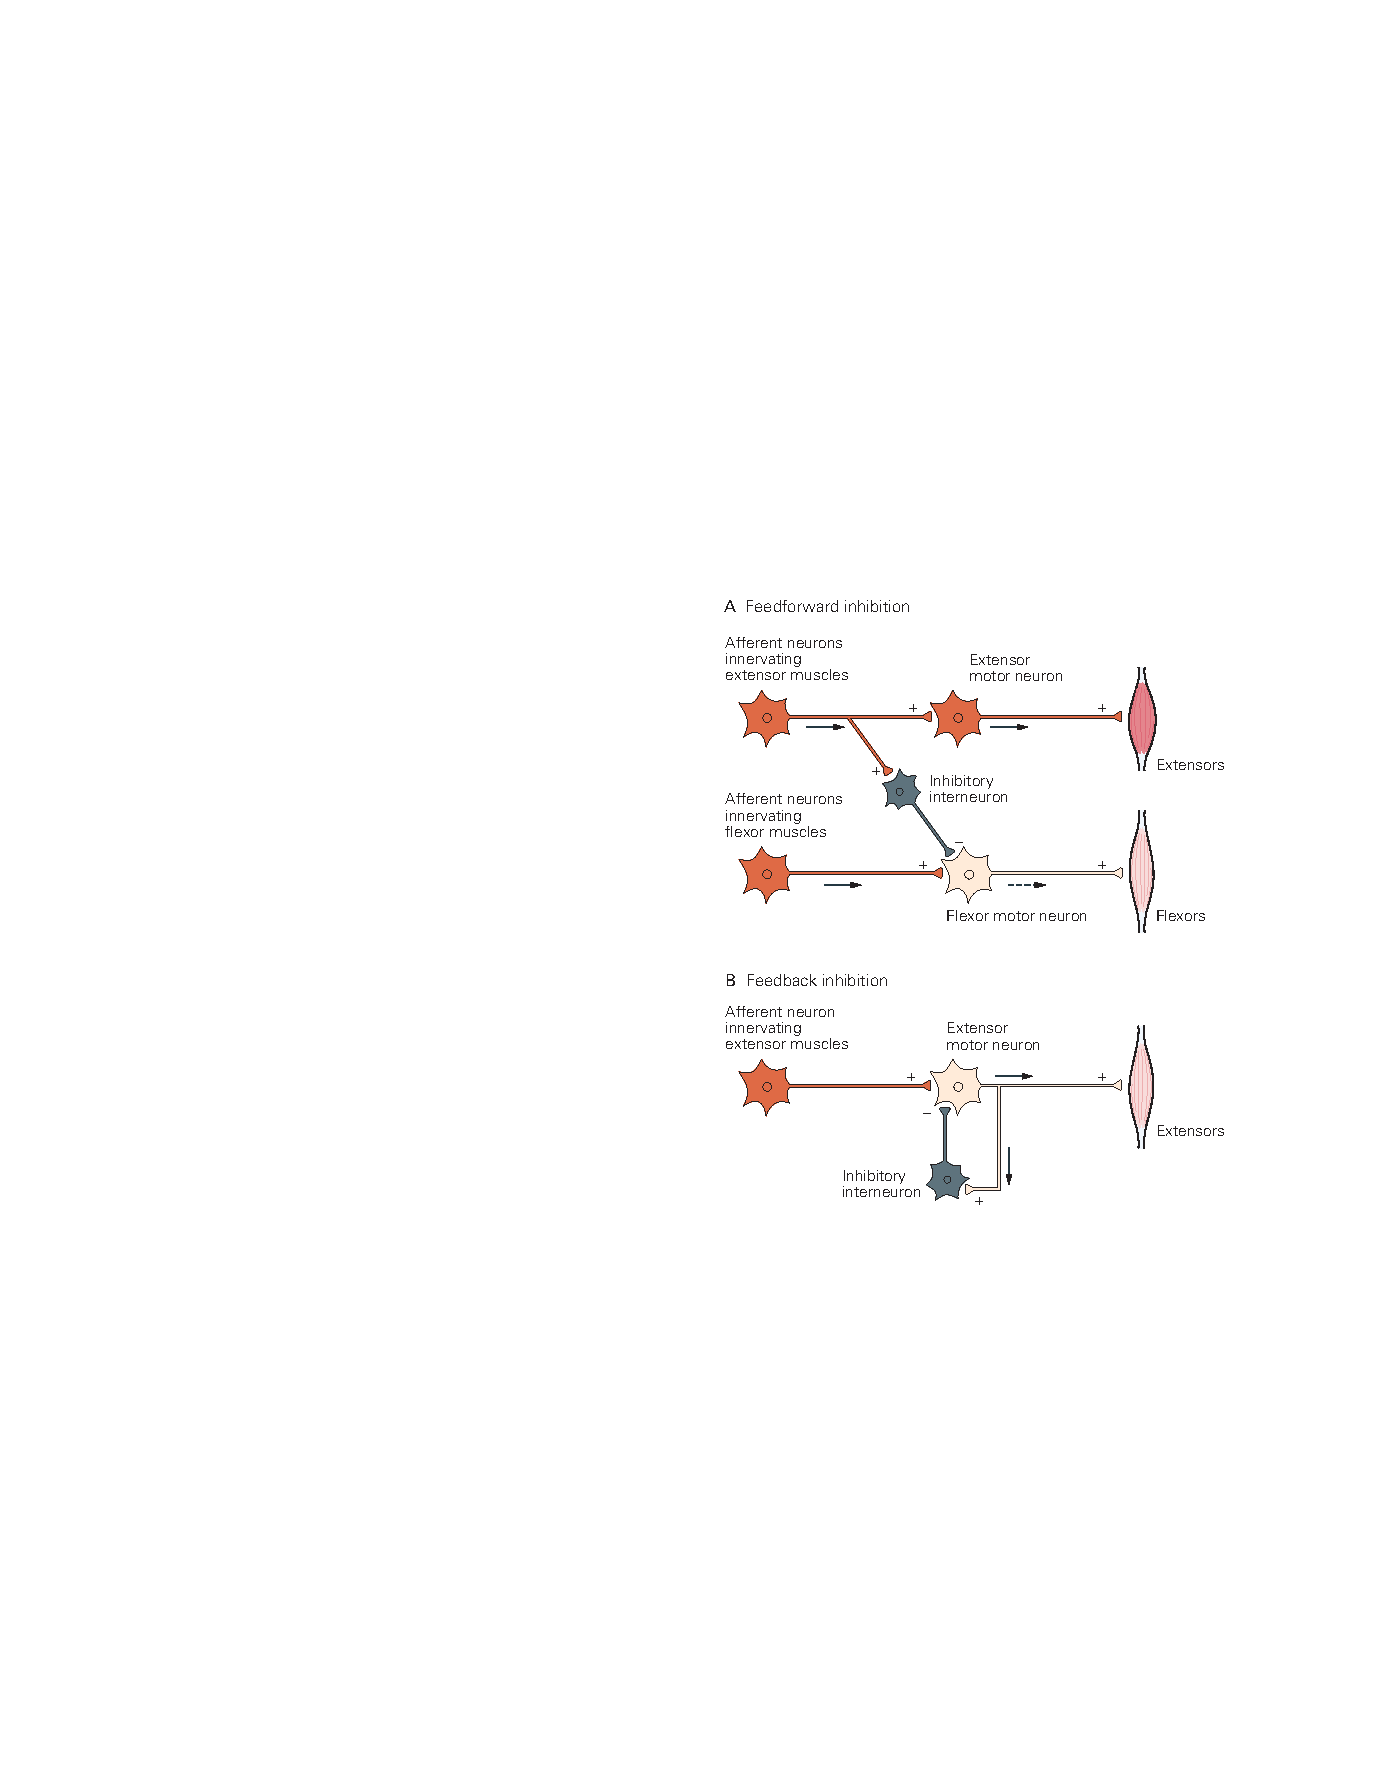
\includegraphics[width=0.5\linewidth]{chap03/fig_3_7}
	\caption{抑制性中间神经元可以产生前馈或反馈抑制。 
		\textbf{A.} 前馈抑制通过抑制调节相反作用的通路的活性来增强活性通路的效果。 
		前馈抑制在单突触反射系统中很常见。 
		例如,在膝跳反射回路(图~\ref{fig:3_5})中,来自伸肌的传入神经元不仅会刺激伸肌运动神经元,还会刺激抑制性中间神经元,从而阻止神经支配相对屈肌的运动细胞的放电。 
		B. 反馈抑制是一种自我调节机制。 
		在这里,伸肌运动神经元作用于抑制性中间神经元,后者反过来作用于伸肌运动神经元本身,从而降低它们放电的可能性。 
		其作用是抑制受刺激通路内的活动并防止其超过某个临界水平。}
	\label{fig:3_7}
\end{figure}


一些回路提供反馈抑制。 
例如,运动神经元可能与肌肉和抑制性中间神经元都有兴奋性连接,后者本身与运动神经元形成连接。 
当抑制性中间神经元被运动神经元兴奋时,中间神经元能够限制运动神经元兴奋肌肉的能力(图 \ref{fig:3_7}B)。 
当我们在后面的章节中研究更复杂的行为时,我们会遇到许多前馈和反馈抑制的例子。


\section{信号在所有神经细胞中的组织方式相同}
为了产生一种行为,例如牵张反射,每个参与的感觉和运动神经细胞必须依次产生四种不同的信号,每个信号位于细胞内的不同位置。 
尽管细胞大小和形状、递质生物化学或行为功能各不相同,但几乎所有神经元都可以用一个模型神经元来描述,该模型神经元具有产生四种类型信号的四个功能组件:
一个用于产生分级输入信号的接收组件,一个求和或 产生触发信号的综合组件,产生全或无传导信号的传导远程信号组件,以及产生输出信号到下一个神经元或肌肉或腺体细胞的突触组件(图 \ref{fig:3_8})。

\begin{figure}[htbp]
	\centering
	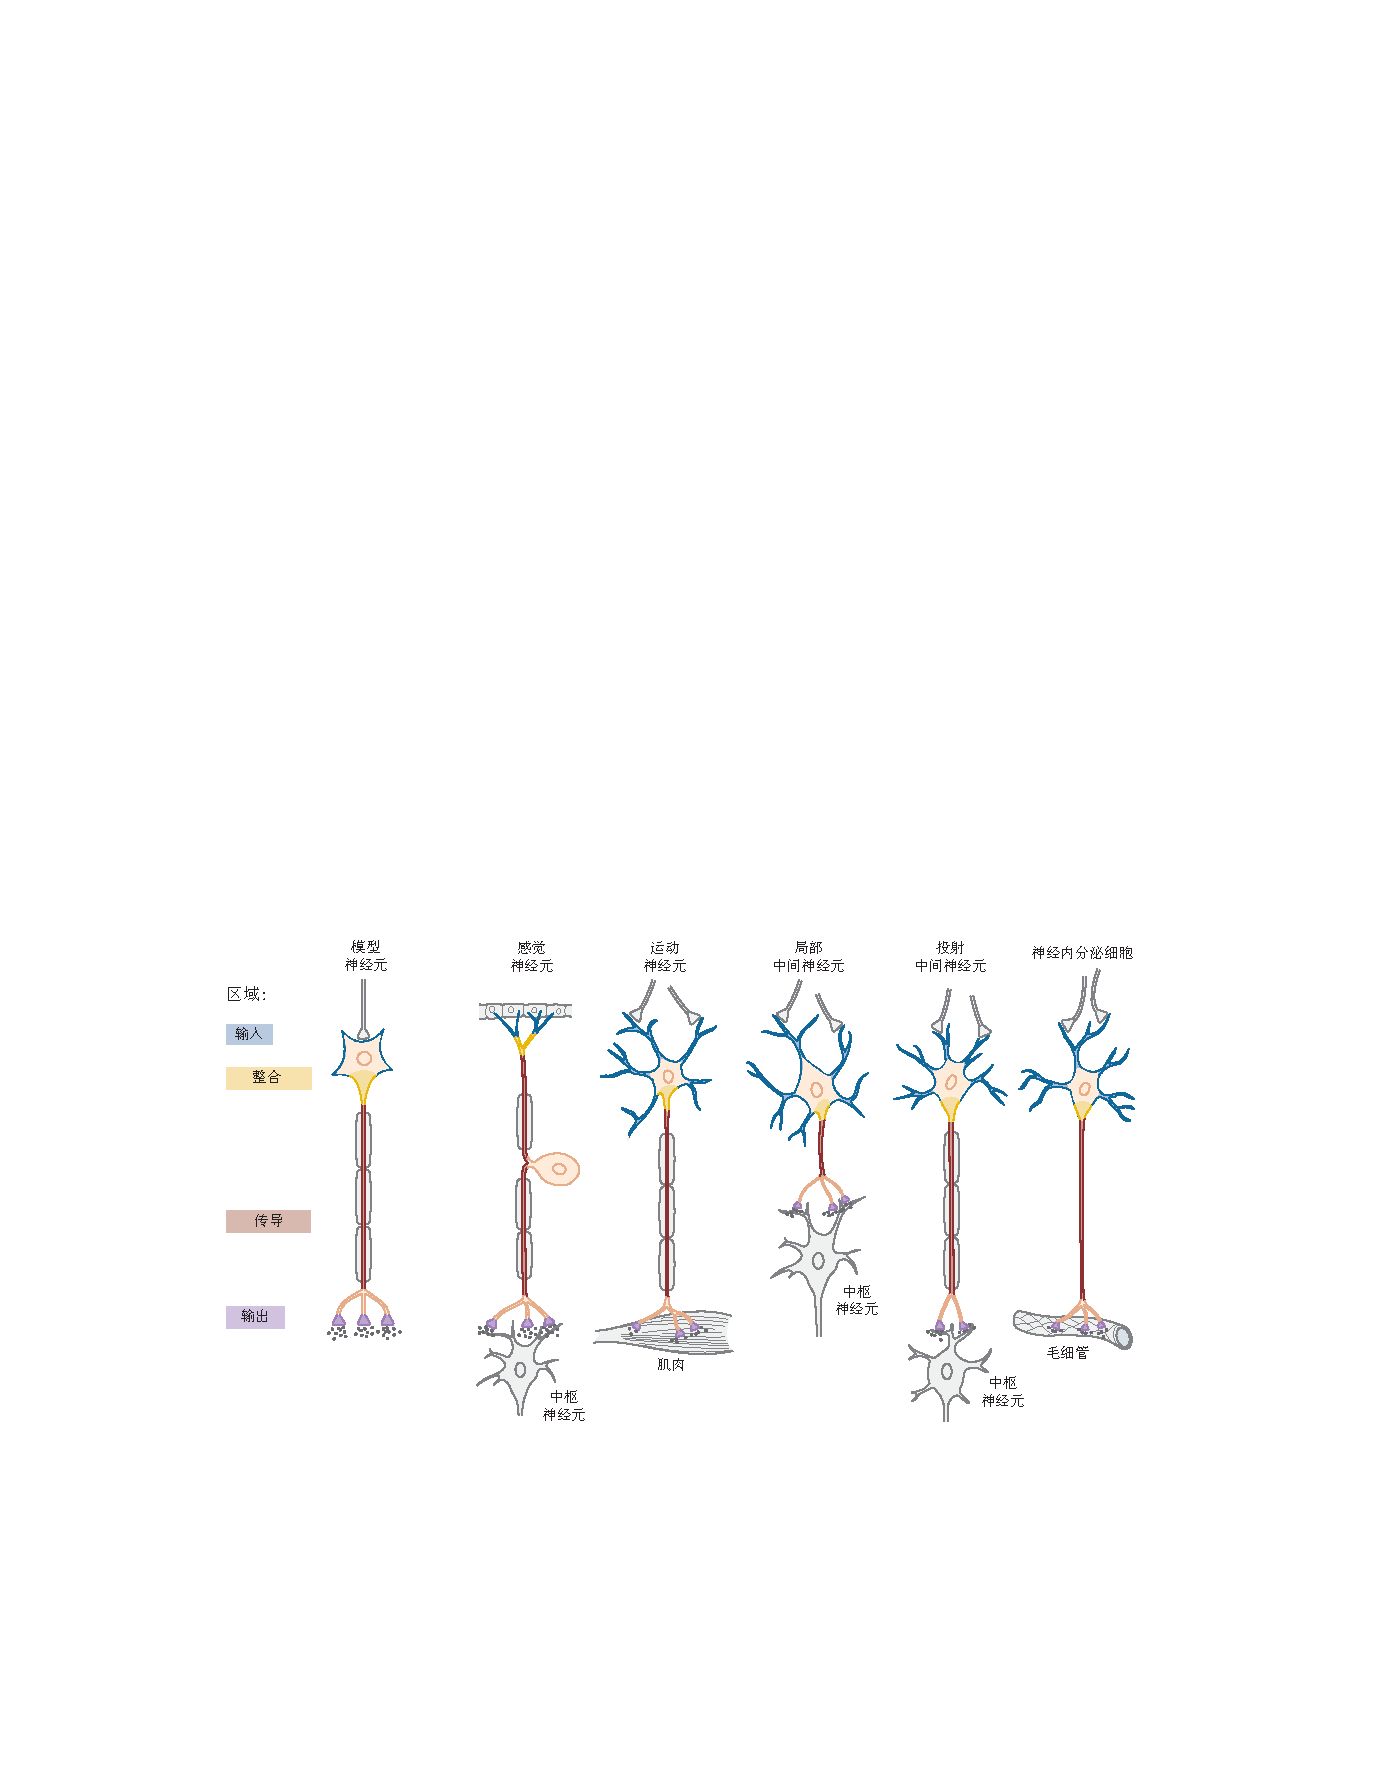
\includegraphics[width=0.5\linewidth]{chap03/fig_3_8}
	\caption{大多数神经元有四个功能区域,在这些区域中会生成不同类型的信号。 
		因此,大多数神经元的功能组织,无论类型如何,都可以用模型神经元示意性地表示。 
		该模型神经元是 Ramón y Cajal 动态极化原理的生理表达。 
		输入信号、综合信号和传导信号都是电信号,对细胞来说是不可或缺的,而输出信号是由细胞射入突触间隙的化学物质。 
		并非所有神经元都具有所有这些特征。 
		例如,一些局部中间神经元缺乏导电成分。}
	\label{fig:3_8}
\end{figure}


神经元中产生的不同类型的信号部分取决于细胞膜的电特性。 
当细胞处于静止状态时,包括神经元在内的每个细胞都在质膜两侧保持一定的电位差。 
这称为静息膜电位。 
在典型的静息神经元中,细胞内部的电压比细胞外部的电压负大约 65 mV。 
因为膜外电压被定义为零,所以我们说静息膜电位为 –65 mV。 
不同神经细胞的静息电位范围为 –40 至 –80 mV; 
在肌肉细胞中,它更大,约为 –90 mV。 
正如第 \ref{chap:chap9} 章中详细描述的,静息膜电位由两个因素造成:带电离子的不均匀分布,特别是带正电的 Na+ 和 \ce{K+},以及膜的选择性渗透性。


带正电的离子在细胞膜两侧的不均匀分布由两个主要机制维持。 
细胞内 Na+ 和 \ce{K+} 浓度主要由膜蛋白控制,膜蛋白主动将 Na+ 泵出细胞并将 \ce{K+} 泵回细胞内。 
这个 Na+-\ce{K+} 泵,我们将在第 \ref{chap:chap9} 章中详细了解,它使细胞内的 Na+ 浓度保持在较低水平(约为细胞外浓度的十分之一),并使 \ce{K+} 浓度保持在较高水平(约为细胞外浓度的 20 倍)。 
Na+ 和 \ce{K+} 的细胞外浓度由肾脏和星形胶质细胞(也称为星形胶质细胞)维持。


否则不可渗透的细胞膜含有形成称为离子通道的孔的蛋白质。 细胞静止时活跃的通道对 \ce{K+} 的渗透性很高,但对 Na+ 的渗透性要低得多。 
\ce{K+} 离子往往会沿着离子的浓度梯度从这些开放通道中泄漏出来。 
当 \ce{K+} 离子离开细胞时,它们会在膜的内表面留下一团未中和的负电荷,因此膜内的净电荷比膜外的负电荷更多。 
在这种情况下,相对于神经元外部,膜电位通常保持在 –65 mV 左右,据说神经元处于静止状态。


当细胞开始吸收细胞外浓度较高的 Na+(或钙离子)时,静息状态就会受到干扰。 
这些带正电的离子向内运动(内向电流)部分地中和了电池内部的负电压。 
我们将在下面详细介绍这些事件。 
然而,接下来发生的事情是理解神经元是什么使信号适合传递信息的关键。


当一个细胞,如神经和肌肉,其膜电位可以迅速而显着地改变时,就被认为是可兴奋的。 
在许多神经元中,膜电位 10 mV 的变化(从 –65 到 –55 mV)使膜对 Na+ 的渗透性比对 \ce{K+} 的渗透性强得多。 
由此产生的 Na+ 流入进一步中和了细胞内的负电荷,导致对 Na+ 的渗透性更高。 
结果是膜电位发生短暂的爆炸性变化,变为 +40 mV,即动作电位。 
这种电位被积极地沿着细胞的轴突传导到轴突的末端,在那里它启动与突触后神经元或肌肉细胞的精细化学相互作用。 
由于动作电位是主动传播的,因此其振幅在到达轴突末端时不会减小。 
动作电位通常持续约 1 毫秒,之后膜恢复到其静止状态,电荷正常分离,对 \ce{K+} 的渗透性高于对 Na+ 的渗透性。


静息电位和动作电位的潜在机制在第 \ref{chap:chap9} 章和第 \ref{chap:chap10} 章中详细讨论。
除了动作电位代表的长距离信号外,神经细胞还产生局部信号——受体电位和突触电位——这些信号不活跃 传播并且通常在几毫米内衰减(见下一节)。


产生远程和局部信号的膜电位变化可以是静息电位的降低或增加。 
也就是说,静息膜电位是所有信号发生的基线。 
膜电位的降低(称为去极化)增强了细胞产生动作电位的能力,因此具有兴奋性。 
相反,膜电位的增加,称为超极化,使细胞不太可能产生动作电位,因此具有抑制作用。


\subsection{输入组件产生分级本地信号}
在大多数静止的神经元中,没有电流从细胞的一部分流向另一部分,因此静息电位始终相同。 
在感觉神经元中,电流通常由物理刺激启动,物理刺激会激活神经元接受表面的特殊受体蛋白。 
在我们膝跳反射的例子中,肌肉的拉伸会激活特定的离子通道,这些离子通道会响应感觉神经元膜的拉伸而打开,我们将在第 \ref{chap:chap18} 章中了解到。
当细胞被拉伸时,这些通道的打开允许 Na+ 离子快速流入感觉细胞。 
这种离子电流改变膜电位,产生称为受体电位的局部信号。


受体电位的幅度和持续时间取决于肌肉拉伸的强度:拉伸越大或持续时间越长,由此产生的受体电位越大或持续时间越长(图 \ref{fig:3_9}A)。 
也就是说,受体电位是分级的,这与 allor-none 动作电位不同。 
大多数受体电位是去极化的(兴奋性的); 在视网膜中发现超极化(抑制)受体电位。

\begin{figure}[htbp]
	\centering
	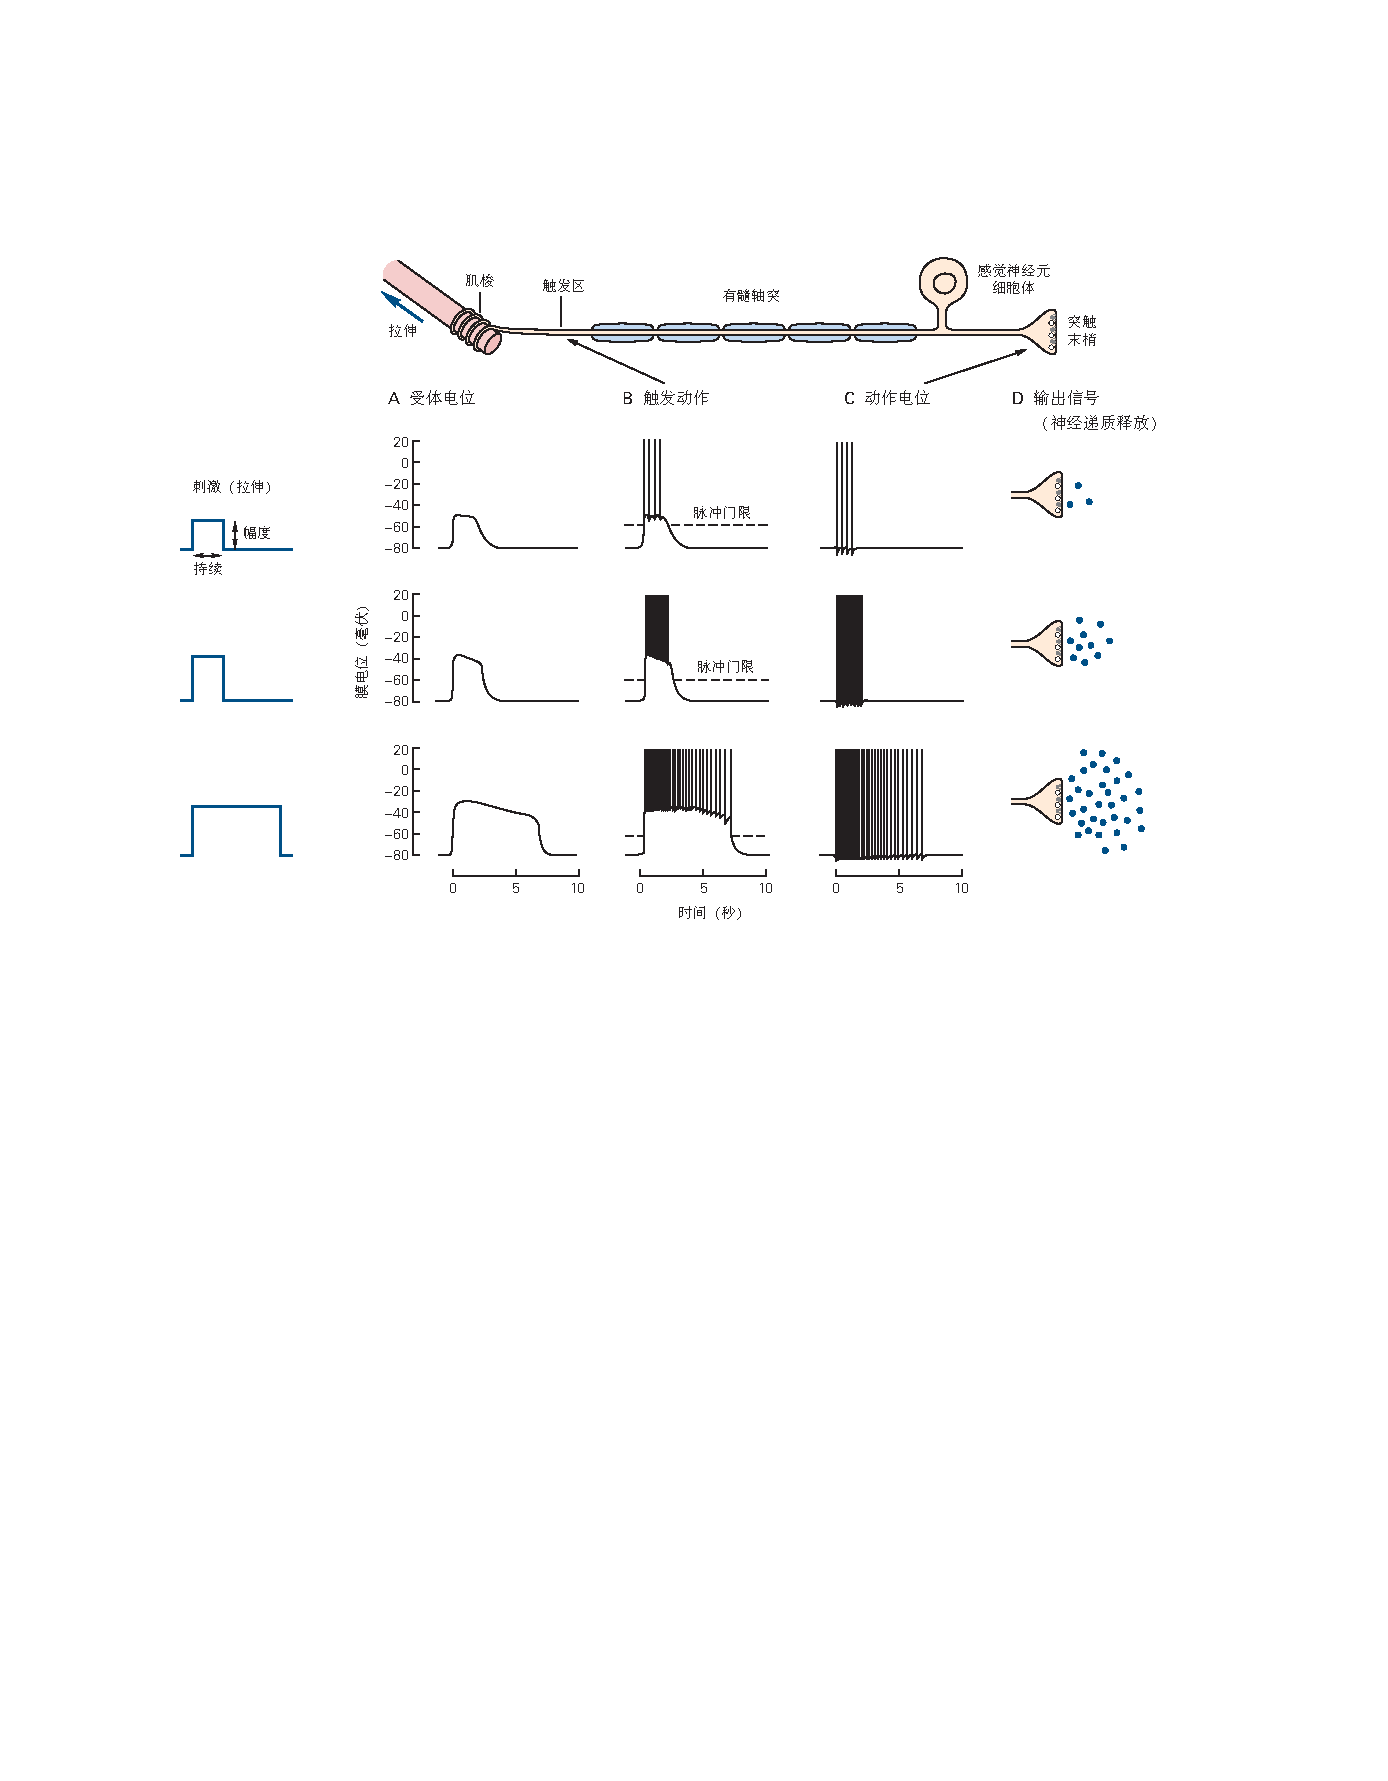
\includegraphics[width=1.0\linewidth]{chap03/fig_3_9}
	\caption{神经元的四个信号成分中的每一个都会产生一个特征信号。 
		该图显示了通过肌肉拉伸激活的感觉神经元,神经元通过专门的受体(肌梭)感知。 
		A. 输入信号,称为受体电位,在振幅和持续时间上分级,与刺激的振幅和持续时间成正比。 
		B. 触发区总结了受体电位产生的去极化。 
		只有当受体电位超过某个电压阈值时才会产生动作电位。 
		一旦超过这个阈值,受体电位幅度的任何进一步增加只能增加动作电位产生的频率,因为动作电位具有恒定的幅度。 
		受体电位的持续时间决定了动作电位序列的持续时间。 
		因此,受体电位的分级振幅和持续时间被转化为触发区产生的动作电位中的频率代码。 
		产生的所有动作电位都忠实地沿着轴突传播。 
		C. 动作电位是全有或全无。 
		因为所有动作电位都具有相似的幅度和持续时间,所以放电的频率和持续时间编码了信号所携带的信息。 
		D. 当动作电位到达突触末梢时,它会启动神经递质的释放,即用作输出信号的化学物质。 
		突触前细胞中动作电位的频率决定了细胞释放多少神经递质。}
	\label{fig:3_9}
\end{figure}

受体电位是在神经系统中编码的第一个拉伸表示。 
然而,由于这种去极化从拉伸感受器被动传播,它不会传播很远。 
如果轴突的直径较大,则距离较长,如果直径较小,则距离较短。 
此外,如果电流可以轻松通过膜,则距离会更短,如果膜被髓磷脂绝缘,则距离会更长。 
因此,来自拉伸感受器的感受器电位仅移动 1 至 2 毫米。 
事实上,就在 1 毫米远的地方,信号的幅度仅为产生位置的三分之一左右。 
为了成功地传送到脊髓,局部信号必须被放大——它必须产生动作电位。 
在膝跳反射中,如果感觉神经元中的受体电位到达轴突中朗飞的第一个节点并且足够大,它将触发动作电位(图 \ref{fig:3_9}B),然后无故障地传播到轴突 脊髓中的末端(图 \ref{fig:3_9}C)。 
在感觉神经元和运动神经元之间的突触处,动作电位会产生一系列事件,这些事件会导致运动神经元的输入信号。


在膝跳反射中,感觉神经元突触前末梢的动作电位启动化学物质或神经递质释放到突触间隙(图 \ref{fig:3_9}D)。 
扩散穿过裂隙后,递质与运动神经元突触后膜中的受体蛋白结合,从而直接或间接打开离子通道。 
随后的电流流动会短暂地改变运动细胞的膜电位,这种变化称为突触电位。


与受体电位一样,突触电位也是分级的; 
它的振幅取决于释放发射器的量。 
在同一细胞中,突触电位可以去极化或超极化,具体取决于被激活的受体分子的类型。 
突触电位,如受体电位,被动传播。 
因此,电位的变化将保持局部,除非信号超出轴突的初始段,在那里它可以产生动作电位。 
一些树突并非完全被动,而是包含促进突触电位的特化,从而提高其产生动作电位的功效(第 \ref{chap:chap13} 章)。 
表 3-1 总结了受体和突触电位的特征。


\subsection{触发区决定产生动作电位}
谢林顿首先指出,神经系统的功能是权衡不同类型信息的后果,然后决定适当的反应。 
神经系统的这种整合功能在神经元触发区(轴突的初始部分)的事件中清晰可见。


动作电位是由 Na+ 通过细胞膜中的通道突然流入而产生的,这些通道响应于膜电位的变化而打开和关闭。 
当输入信号(受体电位或突触电位)使膜区域去极化时,膜电位的局部变化会打开局部 Na+ 通道,使 Na+ 沿着其浓度梯度从 Na+ 浓度高的细胞外流到细胞内 它低的地方。


由于轴突的起始段具有最高密度的电压敏感 Na+ 通道,因此产生动作电位的阈值最低,因此沿细胞膜被动传播的输入信号更有可能在起始段产生动作电位 轴突的部分比在细胞中的其他部位。 
因此,这部分轴突被称为触发区。 
所有受体(或突触)电位的活动都在这里求和,如果输入信号的总和达到阈值,神经元就会产生动作电位。


\subsection{导电成分传播全有或全无动作电位}
动作电位是全有或全无:低于阈值的刺激不会产生信号,但高于阈值的刺激都会产生相同幅度的信号。 
无论刺激强度或持续时间的变化如何,每个动作电位的幅度和持续时间几乎相同,这适用于沿着有髓轴突的朗飞节点处的每个再生动作电位。 
此外,与被动传播和振幅减小的受体和突触电位不同,正如我们所见,动作电位在沿着轴突到达其目标(距离可达 1 米)时不会衰减。 
因为它是周期性再生的。 
这种传导信号可以以高达 100 m/s 的速度传播。 
事实上,动作电位的显着特征是它们是高度刻板的,从一个神经细胞到另一个神经细胞的变化很小(但在某些情况下很重要)。 
埃德加·阿德里安 (Edgar Adrian) 在 1920 年代证明了这一特征,他是最早在细胞水平上研究神经系统的人之一。 
阿德里安发现所有动作电位都具有相似的形状或波形(见图 \ref{fig:3_2})。 
由感觉轴突带入神经系统的动作电位与由运动轴突从神经系统带入肌肉的动作电位通常无法区分。


传导信号只有两个特征传达信息:动作电位的数量和它们之间的时间间隔(图 \ref{fig:3_9}C)。 
正如阿德里安 (Adrian) 在 1928 年总结他对感觉纤维的研究时所说:“所有的冲动都非常相似,无论信息是注定要引起光感、触感还是痛感; 如果它们挤在一起,感觉就会强烈,如果它们相距很远,感觉就会相应地微弱。” 
因此,决定感觉强度或运动速度的是动作电位的频率。 
同样,感觉或运动的持续时间由产生动作电位的时间段决定。


除了动作电位的频率,动作电位的模式也传达了重要的信息。 
例如,一些神经元在没有刺激的情况下会自发活跃。 
一些自发活跃的神经细胞(跳动的神经元)有规律地激发动作电位; 其他人(爆发的神经元)在短暂的动作电位爆发中发射。 
这些不同的细胞对相同的兴奋性突触输入有不同的反应。 
兴奋性突触电位可能会在一个非自发活跃的细胞中启动一个或多个动作电位,而对自发活跃细胞的相同输入只会增加现有的放电率。


当输入信号具有抑制性时,会出现更显着的差异。 抑制性输入在沉默细胞中几乎没有信息价值。 
相比之下,在自发活跃的细胞中,抑制可以起到强大的塑造作用。 
通过在其他正在进行的活动中建立沉默期,抑制可以在不存在的地方产生一种复杂的交替放电和沉默模式。 
放电模式的这种细微差异可能对神经元之间的信息传递产生重要的功能影响。 
神经元网络的数学建模者试图描述神经代码,其中信息也由细粒度的放电模式——每个动作电位的确切时间——携带。


如果信号是固定的并且仅反映刺激的最基本属性,那么它们如何携带复杂行为所需的丰富信息呢? 
如何将包含蜜蜂视觉信息的信息与包含蜜蜂蜇伤疼痛信息的信息区分开来?
这些感觉信号与自主运动的运动信号有何区别? 
答案很简单,但却是神经系统最重要的组织原则之一:
相互连接的神经元形成解剖学和功能上不同的通路——标记线——正是这些连接神经元的通路,这些标记线,而不是单个神经元,传达 信息。 
视网膜中对光有反应的受体细胞激活的神经通路与皮肤中对触觉有反应的感觉细胞激活的神经通路完全不同。


\subsection{输出组件释放神经递质}
当动作电位到达神经元的末端时,它会刺激细胞释放化学物质。 
这些物质称为神经递质,可以是有机小分子,例如 L-谷氨酸和乙酰胆碱,也可以是肽,例如 P 物质或 LHRH(促黄体激素释放激素)。


神经递质分子存在于称为突触小泡的亚细胞器中,突触小泡聚集在轴突末端的特殊释放部位,称为活性区。 
为了将它们的递质物质喷射到突触间隙中,囊泡向上移动并与神经元的质膜融合,然后通过已知的过程突然打开以将递质释放到突触间隙(突触前细胞和突触后细胞之间的细胞外空间)中 作为胞吐作用。 
第 \ref{chap:chap14} 章和第 \ref{chap:chap15} 章描述了神经递质释放的分子机制。


释放的神经递质分子是神经元的输出信号。 
因此,输出信号根据释放的递质量进行分级,递质量由到达突触前末梢的动作电位的数量和频率决定(图 \ref{fig:3_9}C,D)。 
释放后,递质分子扩散穿过突触间隙并与突触后神经元上的受体结合。 
这种结合导致突触后细胞产生突触电位。 
突触电位是否具有兴奋或抑制作用取决于突触后细胞中受体的类型,而不取决于特定的化学神经递质。 
相同的递质物质在不同的受体上可能有不同的作用。


\subsection{牵张反射通路说明了神经信号从感觉到运动的转变}
正如我们所见,当信号从神经元的一个组成部分移动到另一个组成部分或在神经元之间移动时,信号的属性会发生变化。 
在牵张反射中,当肌肉被拉伸时,刺激的幅度和持续时间反映在感觉神经元中产生的受体电位的幅度和持续时间中(图 \ref{fig:3_10}A)。 
如果受体电位超过该细胞中动作电位的阈值,则分级信号会在触发区转换为动作电位。
尽管个体动作电位是全有或全无信号,但受体电位超过阈值越多,去极化越大,因此轴突中动作电位的频率就越高。 
输入信号的持续时间也决定了动作电位序列的持续时间。

\begin{figure}[htbp]
	\centering
	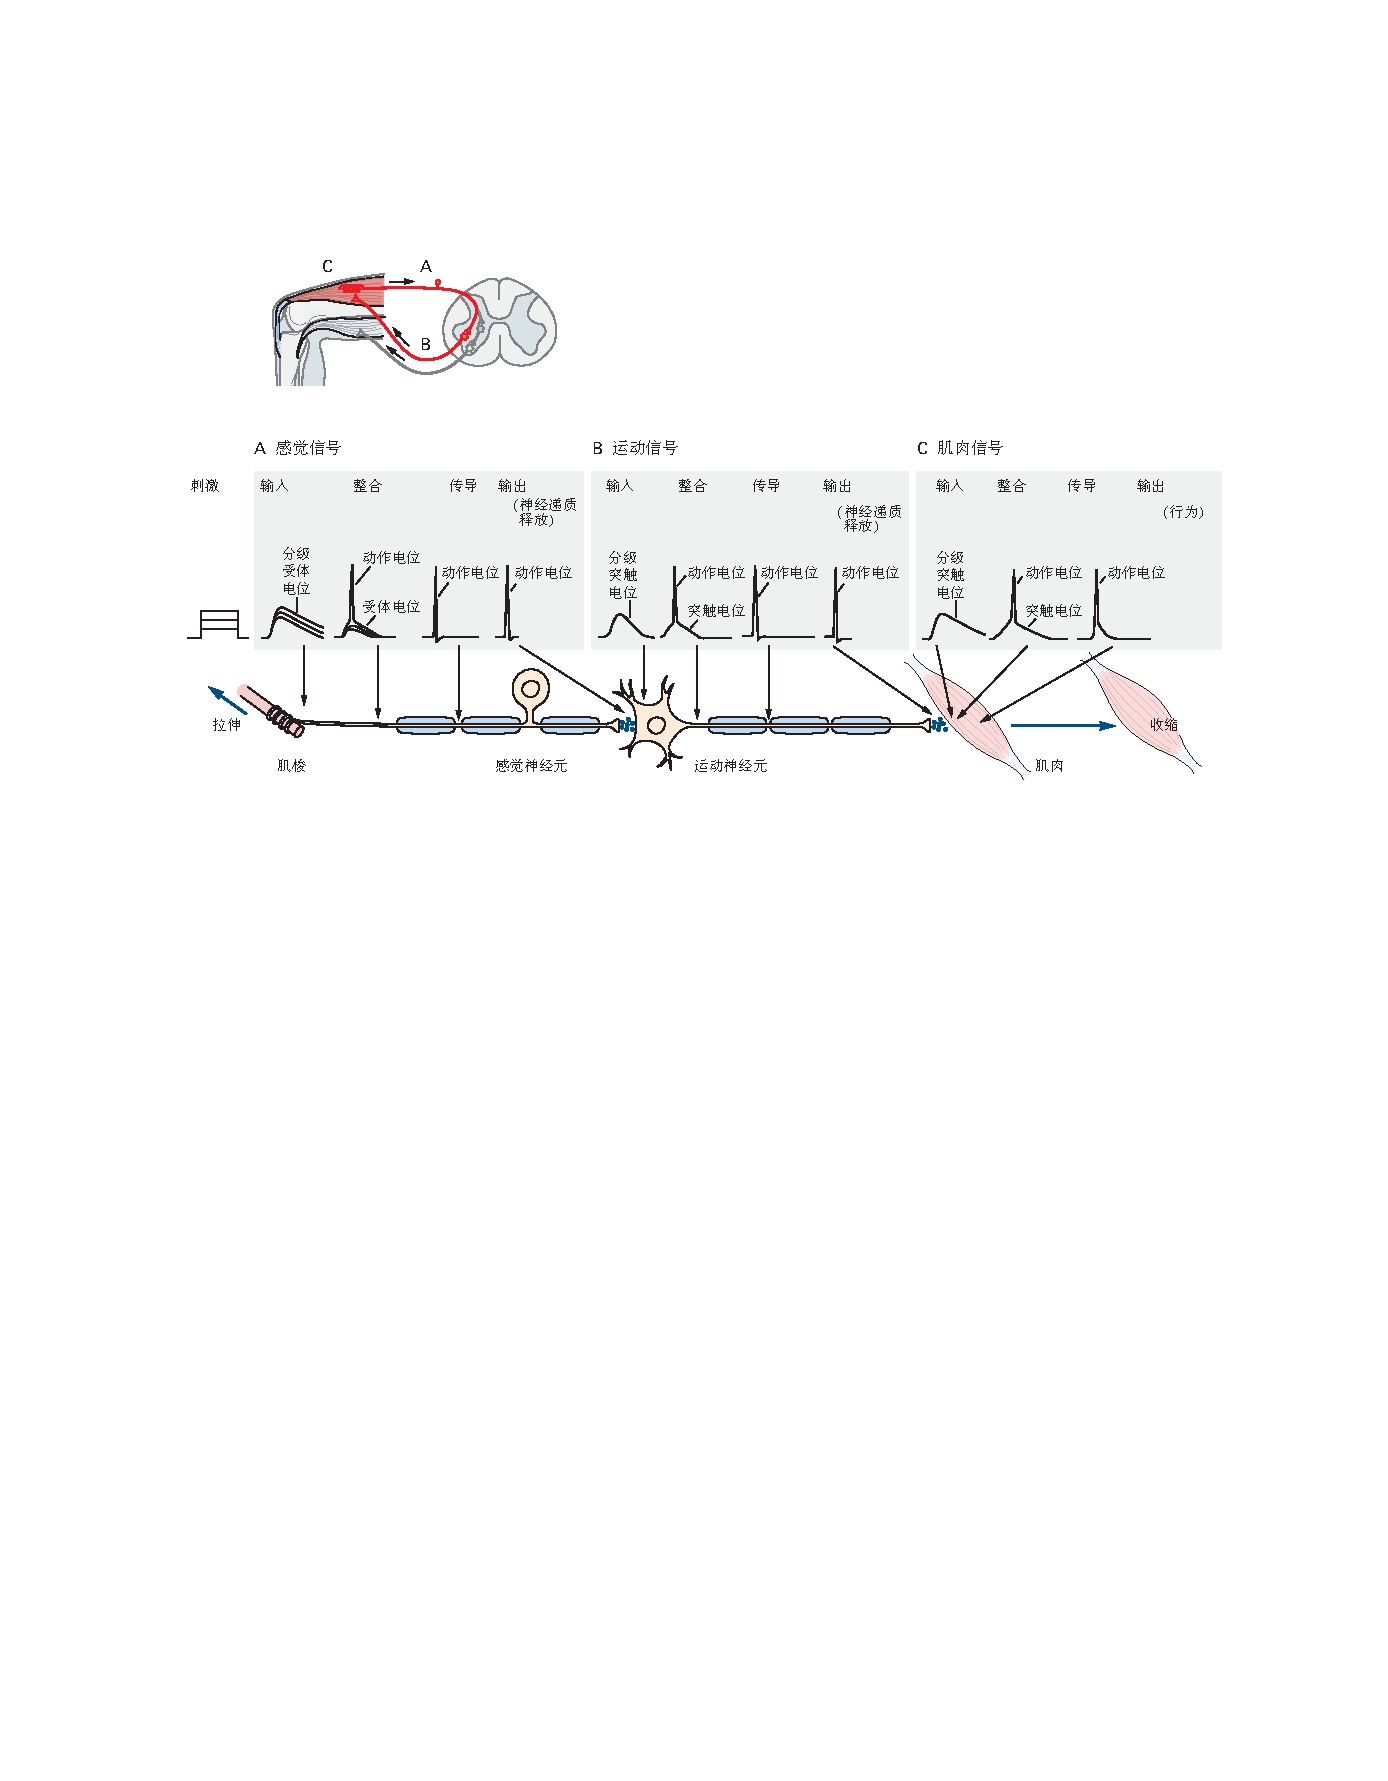
\includegraphics[width=1.0\linewidth]{chap03/fig_3_10}
	\caption{产生反射动作的信号序列。 
		A. 肌肉的拉伸会在专门的受体(肌梭)中产生受体电位。 
		受体电位的幅度与拉伸强度成正比。 
		这种势能被动地传播到朗飞第一个节点的综合区或触发区。 
		如果受体电位足够大,它会触发动作电位,然后沿着轴突主动传播而不会发生变化,直至轴突末端。 
		在终端的特定位置,动作电位导致化学神经递质(输出信号)的释放。 
		递质扩散穿过轴突末端和支配拉伸肌肉的目标运动神经元之间的突触间隙; 
		然后它与运动神经元外膜上的受体分子结合。 
		B. 这种相互作用启动了一个被动传播到运动神经元轴突触发区的突触电位,在那里它启动了一个主动传播到运动神经元轴突末端的动作电位。 
		在轴突末端,动作电位导致肌肉纤维附近神经递质的释放。 
		C. 神经递质结合肌纤维上的受体,产生突触电位。 
		突触电位触发肌肉中的动作电位,从而引起收缩。}
	\label{fig:3_10}
\end{figure}


由放电频率和持续时间编码的信息沿着轴突忠实地传递到其末端,在那里动作电位的放电决定了发射器的释放量。 
这些信号阶段在运动神经元(图 \ref{fig:3_10}B)和肌肉(图 \ref{fig:3_10}C)中有对应的阶段。


\section{神经细胞在分子水平上的差异最大}
我们概述的神经元信号模型是一种适用于大多数神经元的简化模型,但也有一些重要的变化。 
例如,一些神经元不产生动作电位。 
这些通常是没有导电成分的局部中间神经元; 它们没有轴突或轴突太短以至于不需要信号的再生。 
在这些神经元中,输入信号被汇总并被动传播到释放递质附近的突触前末梢区域。 
自发活跃的神经元不需要感觉或突触输入来激发动作电位,因为它们具有一类特殊的离子通道,即使在没有兴奋性突触输入的情况下也允许 Na+ 电流流动。


即使是形态相似的细胞在分子细节上也可能存在重大差异。 
例如,它们可以具有不同的离子通道组合。 
正如我们将在第 \ref{chap:chap10} 章中了解到的,不同的离子通道为神经元提供了不同的阈值、兴奋特性和放电模式。 
这样的神经元可以将突触电位编码成不同的放电模式,从而传达不同的信息。


神经元在用作递质的化学物质和从其他神经元接收递质物质的受体方面也有所不同。 
事实上,许多作用于大脑的药物都是通过改变特定化学递质或受体的作用来实现的。 
由于神经元之间的生理差异,一种疾病可能影响一类神经元而不影响其他神经元。 
某些疾病只影响运动神经元(肌萎缩侧索硬化症和脊髓灰质炎),而其他疾病主要影响感觉神经元(麻风病和脊髓灰质炎,梅毒晚期)。 
帕金森病是一种随意运动障碍,会损害一小部分使用多巴胺作为神经递质的神经元。 
有些疾病甚至在神经元内也具有选择性,仅影响感受元件、细胞体或轴突。 
在第 \ref{chap:chap57} 章中,我们描述了对重症肌无力(一种由肌肉膜中有缺陷的递质受体引起的疾病)的研究如何为突触传递提供了重要的见解。 
事实上,由于神经系统在分子水平上有如此多的细胞类型和变异,它比身体的任何其他器官系统更容易患上更多的疾病(精神病学和神经学)。


尽管神经细胞之间存在形态差异,但电信号的分子机制却惊人地相似。 
这种简单性是幸运的,因为了解一种神经细胞中信号传导的分子机制有助于理解许多其他神经细胞中的这些机制。


\section{反射回路是理解行为神经结构的起点}
牵张反射说明了几种类型的神经细胞之间的相互作用如何构成一个产生简单行为的功能回路,即使涉及的神经元数量很大(牵张反射回路可能有几百个感觉神经元和一百个运动神经元) 神经元)。 
一些无脊椎动物能够使用少得多的神经元做出与反射一样复杂的行为。 
此外,在某些情况下,仅一个关键命令神经元就可以触发复杂的行为,例如从有害刺激中撤回身体部位。


对于更复杂的行为,尤其是高等脊椎动物,需要许多神经元,但通常会保留简单反射的基本神经结构。 
首先,通常有一组可识别的神经元,其放电率会随着特定类型的环境刺激而变化,例如特定频率的音调,或特定角度的明暗并置。 
正如牵张感受器神经元的放电率编码肌肉紧张程度,皮层感觉区域的皮层神经元放电率编码感觉特征的强度(例如,轮廓的对比度)。 
正如我们将在后面的章节中看到的那样,仅通过改变一小组神经元的放电率就可以改变知觉的特征。


其次,通常有一组可识别的神经元,其放电率在动物执行运动动作之前发生变化。 
正如运动神经元的尖峰率控制股四头肌收缩的幅度——因此膝反射——运动皮层神经元的放电率也影响将要进行的运动的潜伏期和类型。 
这些神经元究竟对运动的哪个方面进行了编码仍然是一个活跃的研究领域,但已经确定的是,神经元组通过调整其放电率以分级方式影响随后的动作。 
在大脑皮层的其他关联区域,神经元的分级放电率编码对思维过程至关重要的数量,例如与选择相关的证据数量(第 \ref{chap:chap56} 章)。


尽管复杂的心理操作比简单的牵张反射复杂得多,但考虑认知功能在多大程度上受到以类似于简单反射的任何方式组织的神经机制的支持,可能证明是有用的。 
调解复杂的行为和思想可能需要哪些类型的阐述? 
与具有复杂行为的简单反射不同,感觉神经元的激活不会立即引起反射动作。 
这个过程有更多的偶然性。 
尽管简单的反应受上下文调节,但心理功能更受复杂的突发事件的影响,考虑到任何一种刺激的许多可能影响以及任何一种行为的许多可能的沉淀物。 
鉴于这些突发事件,我们不得不设想在大脑的数据采集系统(不仅是感觉系统,还有记忆系统)和效应器系统之间建立灵活的路由。 
正如我们将在后面的章节中看到的那样,这是大脑皮层的高级联合区域的作用,与几个皮层下脑结构协同作用。


也许复杂的心理功能和反射之间更显着的区别是行动的时机。 
一旦被激活,反射回路几乎会在感官刺激后立即采取行动。 
任何延迟主要取决于反射的传入和传出肢体中动作电位的传导速度(例如,踝反射比膝反射慢,因为脊髓离小腿肌肉的牵张感受器比它离小腿肌肉的牵拉感受器更远) 来自大腿伸肌)。 
对于更复杂的行为,动作不需要随着感官信息的到达而或多或少地立即发生。 它可能会延迟等待其他信息或仅在特定情况发生时才表达。


有趣的是,灵长类动物皮层联合区的神经元有能力在数秒内维持分级放电率。 
这些神经元大量存在于调节感觉和运动区域之间灵活联系的大脑区域。 
它们提供了摆脱反射行为的瞬时性质的自由,因此可以提供将认知功能与更直接的感觉运动转换(如反射)区分开来的基本回路特性。


\section{神经回路可以通过经验进行修改}
学习可以导致持续数年甚至一生的行为改变。 
但即使是简单的反应也可以改变,尽管时间要短得多。 
许多行为可以通过学习来改变这一事实提出了一个有趣的问题:如果神经系统连接得如此精确,那么行为是如何改变的呢? 
当信号单元(神经元)之间的连接在早期发育过程中设置时,行为的神经控制如何发生变化?


针对这一困境,已经提出了几种解决方案。 
最有远见的提议是可塑性假说,该假说由拉蒙·卡哈尔 (Ramón y Cajal) 在 20 世纪之交首次提出。 
波兰心理学家 Jerzy Konorski 于 1948 年提出了这一假设的现代形式。


刺激的应用导致神经系统发生双重变化……[T]第一个特性,神经细胞据此对传入的冲动做出反应……我们称之为兴奋性,并且……由于这个特性而产生变化…… 我们称由于兴奋性而产生的变化。 
第二个属性,由于适当的刺激或它们的组合,特定的神经元系统中会出现某些永久的功能转换,我们将称之为可塑性和相应的变化可塑性变化。


现在有相当多的证据表明化学突触的功能可塑性。 
这些突触通常具有显着的短期生理变化(持续几秒到几小时)的能力,这些变化会增加或减少突触的有效性。 
长期的生理变化(持续数天或更长时间)会引起解剖学改变,包括突触的修剪甚至新突触的生长。 
正如我们将在后面的章节中看到的那样,化学突触在早期发育的关键时期以及整个生命过程中都会在功能和解剖学上发生变化。 
神经元的这种功能可塑性赋予我们每个人与周围自然和社会世界互动的独特方式。



\section{亮点}
1. 神经细胞是神经系统的信号单位。 信号主要是细胞内的电信号和细胞之间的化学信号。 
尽管大小和形状各不相同,但神经细胞具有某些共同特征。 
每个人都有专门的受体或传感器,分别接收来自其他神经细胞或感官的输入; 
一种将输入转换为电信号的机制; 产生全或无电脉冲的阈值机制,即动作电位,可以沿着将神经细胞连接到其突触目标(另一个神经细胞、肌肉或腺体)的轴突再生; 以及产生影响目标的化学物质(神经递质)释放的能力。


2.胶质细胞支持神经细胞。 
一种类型提供绝缘,可加速动作电位沿轴突的传播。 
其他帮助建立神经细胞运作的化学环境,还有一些将神经活动与神经系统的血管供应联系起来。


3. 神经细胞的形态、它们建立的联系以及它们建立的位置不同。 
这在视网膜等特殊结构中最为明显。 
也许神经元之间最大的差异是在分子水平上。 
分子多样性的例子包括不同受体的表达、用于合成不同神经递质的酶以及离子通道的不同表达。 
基因表达的差异为理解为什么某些疾病影响某些神经元而不影响其他神经元提供了起点。


4. 每个神经细胞都是具有一种或多种行为功能的回路的一部分。 
牵张反射回路是一个简单电路的例子,它会产生响应刺激的行为。 
它的简单性掩盖了综合功能,例如放松对抗拉伸肌肉的肌肉。


5. 现代神经科学渴望解释比反射复杂得多的心理过程。 
一个自然的起点是理解必须详细说明回路以支持感觉运动转换的方式,这与反射不同,它是偶然的、灵活的,并且不受制于即时的感觉处理和运动控制。


6. 神经连接可以根据经验进行修改。 
在简单的回路中,这个过程是神经元之间连接强度的简单变化。 
现代神经科学的一个工作假设是,在简单回路中发挥作用的“可塑性”机制在学习更复杂的行为和认知功能方面也发挥着关键作用。


%\section{选读}
%
%\section{参考文献}












